\subsection{\texorpdfstring{关于 \(\lambda^{\#}\) 的另一种解释}{关于 \textbackslash lambda\^{}\{\textbackslash\#\} 的另一种解释}}

对于每个 \(x \in X\)，从 H 到 X 的映射 \(\xi \mapsto x\xi\) 是 逆紧的（GT, III, §4, No.~2, Prop. 4），因此 \(\beta\) 在此映射下在 X 上有一个像测度，该像测度集中于轨道 xH（Ch. V, §6, No.~2, Cor. 3 of Prop. 2）；由于 \(\beta\) 左不变，这个像测度只依赖于 x 在 X/H 中的类 \(u = \pi(x)\)，记作 \(\beta_{u}\)。按定义，对于 \(f \in \mathcal{K}(X)\)，

\[
\int_ {\mathrm{X}} f (y) d \beta_ {u} (y) = \int_ {\mathrm{H}} f (x \xi) d \beta (\xi) = f ^ {\flat} (u).\tag{8}
\]

由此可见

\[
(\varepsilon_ {u}) ^ {\sharp} = \beta_ {u}.\tag{9}
\]

引理 2. --- 设 \(f\) 是 \(X\) 上的函数，取值于一个拓扑空间。

\begin{enumerate}
\def\labelenumi{\alph{enumi})}
\tightlist
\item
  若 \(f\) 是一个 \(\geqslant 0\) 的数值函数，则对于 \(x \in X\)，
\end{enumerate}

\[
\int_ {X} ^ {*} f (y) d \beta_ {\dot {x}} (y) = \int_ {H} ^ {*} f (x \xi) d \beta (\xi) \quad (\dot {x} = \pi (x)).
\]

\begin{enumerate}
\def\labelenumi{\alph{enumi})}
\setcounter{enumi}{1}
\item
  \(f\) 为 \(\beta_{\dot{x}}\)-可测的充要条件是，函数 \(\xi \mapsto f(x\xi)\) 在 \(H\) 上为 \(\beta\)-可测的。
\item
  设 \(\mathbf{f}\) 是 \(\mathbf{X}\) 上的函数，取值于 Banach 空间或 \(\overline{\mathbf{R}}\)；则，\(\mathbf{f}\) 为 \(\beta_{\dot{x}}\)-可积（分别为本质上 \(\beta_{\dot{x}}\)-可积）的充要条件是，函数 \(\xi \mapsto \mathbf{f}(x\xi)\) 在 \(\mathbf{H}\) 上为 \(\beta\)-可积（分别为本质上 \(\beta\)-可积）；在此情形下，\(\int_{\mathbf{X}} \mathbf{f}(y) d\beta_{\dot{x}}(y) = \int_{\mathbf{H}} \mathbf{f}(x\xi) d\beta(\xi)\)。
\end{enumerate}

这由 Ch. V, §4, Prop. 2、Prop. 3 和 Th. 2 得出。

由于 \(f^{\flat} \in \mathcal{K}(X/H)\) 对 \(f \in \mathcal{K}(X)\) 成立，公式 (8) 证明了：映射 \(u \mapsto \beta_{u}\) 从 X/H 到 \(\mathcal{M}(X)\) 是弱连续的；族 \((\beta_{u})\) 是 \(\lambda\)-适合的 \(^{1}\)，对于 X/H 上任意正测度 \(\lambda\)；并且

\[
\lambda^ {\sharp} = \int_ {\mathrm{X/H}} \beta_ {u} d \lambda (u),\tag{10}
\]

这给出了 \(\lambda^{\sharp}\) 的一种新解释。

命题 5. --- 设 \(\lambda\) 是 X/H 上的正测度。

\begin{enumerate}
\def\labelenumi{\alph{enumi})}
\item
  设 \(f\) 是一个 \(\lambda^{\sharp}\)-可测函数，定义在 \(X\) 上，取值于一个拓扑空间，并且在某个 \(\lambda^{\sharp}\)-可积集的可数并之外为常值。则那些 \(\dot{x} \in X / H\) 使函数 \(\xi \mapsto f(x\xi)\) 不是 \(\beta\)-可测的点所成的集合是局部 \(\lambda\)-可忽略的。
\item
  设 \(f\) 是一个 \(\lambda^{\sharp}\)-可测的 \(\geqslant 0\) 函数，定义在 \(X\) 上，并在某个 \(\lambda^{\sharp}\)-可积集的可数并之外为零。则函数 \(\dot{x} \mapsto \int^{*} f(x\xi) d\beta(\xi)\) 在 \(X / H\) 上是 \(\lambda\)-可测的，并且
\end{enumerate}

\[
\int_ {\mathrm{X}} ^ {*} f (x) d \lambda^ {\sharp} (x) = \int_ {\mathrm{X/H}} ^ {*} d \lambda (\dot {x}) \int_ {\mathrm{H}} ^ {*} f (x \xi) d \beta (\xi) \qquad \big (\dot {x} = \pi (x) \big).
\]

\begin{enumerate}
\def\labelenumi{\alph{enumi})}
\setcounter{enumi}{2}
\tightlist
\item
  设 \(\mathbf{f}\) 是一个 \(\lambda^{\sharp}\)-可积函数，定义在 \(X\) 上，取值于 Banach 空间或 \(\overline{\mathbf{R}}\)。则那些 \(\dot{x} \in X / H\) 使得函数 \(\xi \mapsto \mathbf{f}(x\xi)\) 不是 \(\beta\)-可积的点所成的集合是 \(\lambda\)-可忽略的；由下式几乎处处定义的函数 \(\mathbf{f}^{\flat}\) 在 \(X / H\) 上
\end{enumerate}

\[
\mathbf {f} ^ {\flat} (\dot {x}) = \int_ {\mathrm{H}} \mathbf {f} (x \xi) d \beta (\xi) \quad \left(\dot {x} = \pi (x)\right)\tag{11}
\]

是 \(\lambda\)-可积的，并且

\[
\int_ {\mathrm{X/H}} \mathbf {f} ^ {\flat} d \lambda = \int_ {\mathrm{X}} \mathbf {f} d \lambda^ {\sharp}\tag{12}
\]

以及

\[
\int_ {\mathrm{X} / \mathrm{H}} | \mathbf {f} ^ {\flat} | d \lambda \leqslant \int_ {\mathrm{X}} | \mathbf {f} | d \lambda^ {\sharp}.\tag{13}
\]

\begin{enumerate}
\def\labelenumi{\alph{enumi})}
\setcounter{enumi}{3}
\tightlist
\item
  设 \(\mathbf{f}\) 是一个 \(\lambda^{\sharp}\)-可测函数，定义在 \(\mathbf{X}\) 上，取值于 \(\overline{\mathbf{R}}\) 或 Banach 空间，并且在某个 \(\lambda^{\sharp}\)-可积集的可数并之外为零。则 \(\mathbf{f}\) 为 \(\lambda^{\sharp}\)-可积的充要条件是
\end{enumerate}

\[
\int_ {\mathrm{X} / \mathrm{H}} ^ {*} d \lambda (\dot {x}) \int_ {\mathrm{H}} ^ {*} | \mathbf {f} (x \xi) | d \beta (\xi) <   + \infty \quad \left(\dot {x} = \pi (x)\right).
\]

结合引理 2，断言 a)、b) 和 c) 由 Ch. V, §3, Prop. 4、Prop. 5 和 Th. 1 得出（(13) 除外；(13) 由 (12) 得出，因为显然有 \(|\mathbf{f}^{\flat}| \leqslant |\mathbf{f}|^{\flat}\)）；d) 由 b) 得出。

命题 6. --- 设 \(\lambda\) 是 X/H 上的正测度。

\begin{enumerate}
\def\labelenumi{\alph{enumi})}
\item
  设 N 是 X/H 的子集。N 局部 \(\lambda\)-可忽略的充要条件是，\(\overline{\pi}^{-1}(N)\) 局部 \(\lambda^{\sharp}\)-可忽略。
\item
  设 \(g\) 是 \(\mathrm{X / H}\) 上取值于一个拓扑空间的函数。\(g\) 为 \(\lambda\)-可测的充要条件是 \(g \circ \pi\) 为 \(\lambda^{\sharp}\)-可测的。
\item
  设 \(\mathbf{h}\) 是 \(\mathrm{X / H}\) 上取值于 Banach 空间或 \(\overline{\mathbf{R}}\) 的函数。\(\mathbf{h}\) 局部 \(\lambda\)-可积的充要条件是 \(\mathbf{h} \circ \pi\) 局部 \(\lambda^{\sharp}\)-可积；在此情形下，\((\mathbf{h} \cdot \lambda)^{\sharp} = (\mathbf{h} \circ \pi) \cdot \lambda^{\sharp}\)。
\end{enumerate}

假设 \(\mathbf{h} \circ \pi\) 局部 \(\lambda^{\sharp}\)-可积。对于每个 \(f \in \mathcal{K}(X)\)，\(f \cdot (\mathbf{h} \circ \pi)\) 都是 \(\lambda^{\sharp}\)-可积的，因此由 Prop. 5，函数 \((f \cdot (\mathbf{h} \circ \pi))^b = f^b \cdot \mathbf{h}\) 是 \(\lambda\)-可积的，并且

\[
\int_ {\mathrm{X} / \mathrm{H}} f ^ {\flat} \cdot \mathbf {h} d \lambda = \int_ {\mathrm{X}} f \cdot (\mathbf {h} \circ \pi) d \lambda^ {\sharp}.
\]

由于 \(f \mapsto f^{\flat}\) 是从 \(\mathcal{K}(\mathrm{X})\) 到 \(\mathcal{K}(\mathrm{X}/\mathrm{H})\) 上的满射，这表明 \(\mathbf{h}\) 局部 \(\lambda\)-可积，并且

\[
(\mathbf {h} \cdot \lambda) ^ {\sharp} = (\mathbf {h} \circ \pi) \cdot \lambda^ {\sharp}.
\]

特别地，若 \(\overline{\pi}^{1}(N)\) 局部 \(\lambda^{\sharp}\)-可忽略，则 \(\varphi_{N} \circ \pi\) 局部 \(\lambda^{\sharp}\)-可忽略，因此 \((\varphi_{N} \cdot \lambda)^{\sharp} = (\varphi_{N} \circ \pi) \cdot \lambda^{\sharp} = 0\)，从而 \(\varphi_{N} \cdot \lambda = 0\)，且 \(N\) 局部 \(\lambda\)-可忽略。现在假设 \(g \circ \pi\) 是 \(\lambda^{\sharp}\)-可测的。设 \(K'\) 是 \(X/H\) 的紧子集。取 \(f \in \mathcal{K}_{+}(X)\)，使得 \(f^{\flat} = 1\) 在 \(K'\) 上（No.~1, Prop. 2），并令 \(K = \operatorname{Supp} f\)；有 \(\pi(K) \supset K'\)。存在 \(K\) 的一个分割，它由一个 \(\lambda^{\sharp}\)-可忽略集 \(M\) 和紧集序列 \((K_n)\) 构成，使得 \((g \circ \pi)|K_n\) 连续，对每个 \(n\) 成立。于是 \(g|\pi(K_n)\) 连续。令 \(P\) 为 \(K'\) 中不属于 \(\pi(K_1) \cup \pi(K_2) \cup \ldots\) 的点集；则 \(\overline{\pi}^{1}(P) \cap K\) 包含于 \(M\) 中，因而是 \(\lambda^{\sharp}\)-可忽略的；所以 \(f \cdot \varphi_{\overline{\pi}(P)}^{-1}\) 是 \(\lambda^{\sharp}\)-可忽略的；由此（Prop. 5）可得

\[
0 = \int_ {\mathrm{X}} f \cdot \varphi_ {\pi^ {- 1} (\mathrm{P})} d \lambda^ {\sharp} = \int_ {\mathrm{X/H}} f ^ {\flat} \cdot \varphi_ {\mathrm{P}} d \lambda \geqslant \int_ {\mathrm{X/H}} ^ {*} \varphi_ {\mathrm{P}} d \lambda ,
\]

因此 \(\mathbf{P}\) 是 \(\lambda\)-可忽略的，且 \(g\) 是 \(\lambda\)-可测的。

若 N 局部 \(\lambda\)-可忽略，则 \(\overline{\pi}^{1}(N)\) 局部 \(\lambda^{\sharp}\)-可忽略（Ch. V, §6, No.~6, Cor. 1 of Prop. 10）。若 g 是 \(\lambda\)-可测的，则 \(g \circ \pi\) 是 \(\lambda^{\sharp}\)-可测的（同上）。最后，假设 h 局部 \(\lambda\)-可积。我们已经知道 \(h \circ \pi\) 是 \(\lambda^{\sharp}\)-可测的。对于每个 \(f \in \mathcal{K}_{+}(X)\)，由 Prop. 5 有

\[
\int_ {X} ^ {*} f (x) | \mathbf {h} | (\pi (x)) d \lambda^ {\sharp} (x) = \int_ {X / H} ^ {*} | \mathbf {h} | (u) f ^ {\flat} (u) d \lambda (u) <   + \infty ,
\]

因此 \(\mathbf{h} \circ \pi\) 局部 \(\lambda^{\sharp}\)-可积。

推论 1. --- 设 \(\lambda, \lambda'\) 是 X/H 上的两个正测度。\(\lambda'\) 以 \(\lambda\) 为基的充要条件是 \(\lambda'^{\sharp}\) 以 \(\lambda^{\sharp}\) 为基。\(\lambda\) 与 \(\lambda'\) 等价的充要条件是 \(\lambda^{\sharp}\) 与 \(\lambda'^{\sharp}\) 等价。

第一个断言由 Prop. 6 的 a) 和 c) 得出。第二个断言由第一个断言得出。

推论 2. --- 设 \(\lambda\) 是 X/H 上的正测度，并设 \(f\) 是 X 上的 \(\lambda^{\sharp}\)-可测数值函数。假设对于每个 \(\xi \in H\)，都有 \(\delta(\xi)f = f\) 局部 \(\lambda^{\sharp}\)-几乎处处成立。则存在 X/H 上的 \(\lambda\)-可测函数 \(g\)，使得 \(f = g \circ \pi\) 局部 \(\lambda^{\sharp}\)-几乎处处成立。

将 \(f\) 替换为 \(f / (1 + |f|)\) 后，可归结为 \(f\) 有界的情形，因而局部 \(\lambda^{\sharp}\)-可积。令 \(\mu = f \cdot \lambda^{\sharp}\)。关于 \(f\) 的假设蕴含，有 \(\pmb{\delta}(\xi) \mu = f \cdot \pmb{\delta}(\xi) \lambda^{\sharp} = \Delta_{\mathrm{H}}(\xi) \mu\)，对于所有 \(\xi \in \mathrm{H}\) 成立。于是存在（Prop. 4）\(\lambda'\)，它是 \(\mathrm{X} / \mathrm{H}\) 上的测度，使得 \(\mu = \lambda'^{\sharp}\)。由推论 1，关于 \(\lambda\)，存在函数 \(g\)，它定义在 \(\mathrm{X} / \mathrm{H}\) 上且局部可积，使得 \(\lambda' = g \cdot \lambda\)。由 Prop. 6，\(f \cdot \lambda^{\sharp} = \lambda'^{\sharp} = (g \circ \pi) \cdot \lambda^{\sharp}\)，从而 \(f = g \circ \pi\) 局部 \(\lambda^{\sharp}\)-几乎处处成立。

推论 3. --- a) 设 \((\lambda_{\iota})_{\iota \in I}\) 是 X/H 上的实测度族。族 \((\lambda_{\iota})\) 在 \(\mathcal{M}(\mathrm{X / H})\) 中有上界的充要条件是族 \((\lambda_{\iota}^{\sharp})\) 在 \(\mathcal{M}(\mathrm{X})\) 中有上界；在此情形下

\[
\sup (\lambda_ {\iota} ^ {\sharp}) = (\sup \lambda_ {\iota}) ^ {\sharp}.
\]

\begin{enumerate}
\def\labelenumi{\alph{enumi})}
\setcounter{enumi}{1}
\item
  设 \(\lambda\) 是 X/H 上的实测度。则 \((\lambda^{+})^{\sharp} = (\lambda^{\sharp})^{+}\)，且 \((\lambda^{-})^{\sharp} = (\lambda^{\sharp})^{-}\)。
\item
  设 \(\lambda\) 是 X/H 上的复测度。则 \(|\lambda|^{\sharp} = |\lambda^{\sharp}|\)。
\end{enumerate}

假设族 \((\lambda_{\iota})\) 有上界，并令 \(\mu = \sup \lambda_{\iota}\)。由于 \(\lambda \geqslant 0\) 蕴含 \(\lambda^{\sharp} \geqslant 0\)，故有 \(\mu^{\sharp} \geqslant \lambda_{\iota}^{\sharp}\)，对所有 \(\iota\) 成立，这表明族 \((\lambda_{\iota}^{\sharp})\) 有上界，并且

\[
(\sup \lambda_ {\iota}) ^ {\sharp} \geqslant \sup (\lambda_ {\iota} ^ {\sharp}).
\]

反之，假设族 \((\lambda_{\iota}^{\sharp})\) 有上界，并令 \(\nu = \sup(\lambda_{\iota}^{\sharp})\)。由于有 \(\delta(\xi)\lambda_{\iota}^{\sharp} = \Delta_{\mathrm{H}}(\xi)\lambda_{\iota}^{\sharp}\)，对于所有 \(\xi \in H\) 成立，显然 \(\delta(\xi)\nu = \Delta_{\mathrm{H}}(\xi)\nu\)，因此存在 \(\mu' \in \mathcal{M}(\mathrm{X}/\mathrm{H})\)，使得 \(\nu = \mu'^{\sharp}\)。由于 \(\lambda^{\sharp} \geqslant 0\) 蕴含 \(\lambda \geqslant 0\)，故 \(\mu' \geqslant \lambda_{\iota}\)，对所有 \(\iota\) 成立，这表明族 \((\lambda_{\iota})\) 有上界，并且 \(\nu = \mu'^{\sharp} \geqslant (\sup \lambda_{\iota})^{\sharp}\)，从而

\[
\sup \left(\lambda_ {\iota} ^ {\sharp}\right) \geqslant \left(\sup \lambda_ {\iota}\right) ^ {\sharp},
\]

这就完成了 a) 的证明。b) 的断言立即得出，因为例如 \(\lambda^{+}\) 正是 \(\sup(\lambda,0)\)。为证明 c)，只需注意，\(|\lambda| = \sup \mathcal{R}(\alpha \lambda)\)，其中上确界取遍绝对值为 1 的复数 \(\alpha\)；另一方面，\(\mathcal{R}(\mu^{\sharp}) = (\mathcal{R}\mu)^{\sharp}\) 对于每个 \(\mu \in \mathcal{M}(\mathrm{X / H})\) 成立。

注记。--- 1) Prop. 6 a) 可表述为：\(\lambda\) 是 \(\lambda^{\sharp}\) 在 \(\pi\) 下的拟像测度（Ch. VI, §3, No.~2, Def. 1）。

\begin{enumerate}
\def\labelenumi{\arabic{enumi})}
\setcounter{enumi}{1}
\tightlist
\item
  假设 H 紧且 \(\beta\) 已归一化。X 的每个紧子集的饱和集都是紧的。因此，若 \(f \in \mathcal{K}(\mathrm{X}/\mathrm{H})\)，则 \(f \circ \pi \in \mathcal{K}(\mathrm{X})\)；并且对于 X/H 上的每个正测度 \(\lambda\)，Prop. 5 c) 给出
\end{enumerate}

\[
\int_ {\mathrm{X}} (f \circ \pi) (x) d \lambda^ {\sharp} (x) = \int_ {\mathrm{X/H}} f (u) d \lambda (u).
\]

换言之，\(\lambda\) 是 \(\lambda^{\sharp}\) 在 \(\pi\) 下的像测度。

\begin{enumerate}
\def\labelenumi{\arabic{enumi})}
\setcounter{enumi}{2}
\item
  Prop. 6 的 Cor. 3 c) 立即表明，本小节的结果在复测度情形仍然成立（涉及上积分的结果除外）。
\item
  设 \(\mathbf{m}\) 是 X/H 上取值于 E 的向量测度，且 \(q\) 是 E 上的下半连续半范数。\(\mathbf{m}\) 为 \(q\)-可控的（Ch. VI, §2, No.~3, Def. 3）的充要条件是 \(\mathbf{m}^{\sharp}\) 具有同样性质；在此情形下 \(q(\mathbf{m}^{\sharp}) = q(\mathbf{m})^{\sharp}\)。这立即由定义和 Cor. 3 a) 得出。
\end{enumerate}

另一方面，设 \(\mu\) 是 X/H 上的正测度。m 按标量以 \(\mu\) 为基的充要条件是 \(\mathbf{m}^{\sharp}\) 按标量以 \(\mu^{\sharp}\) 为基；这由 Cor. 1 得出。

最后，若 \(\mathbf{m}\) 以 \(\mu\) 为基，并且密度为 \(\mathbf{f}\)（关于 \(\mu\)，Ch. VI, §2, No.~4, Def. 4），则 \(\mathbf{m}^{\sharp}\) 以 \(\mu^{\sharp}\) 为基，密度为 \(\mathbf{f} \circ \pi\)：这由 Prop. 6 c) 得出。

\subsection{X/H 仿紧的情形}

若 X/H 是仿紧的，我们先来考察：向量空间 \(\mathcal{K}^{\chi}(X)\)（其中 \(\chi\) 变动）彼此同构，特别地都与 \(\mathcal{K}^{1}(X)\) 同构。

命题 7. --- 假设 X/H 仿紧。设 \(\chi\) 是 H 到 \(\mathbf{R}_{+}^{*}\) 的连续表示。

\begin{enumerate}
\def\labelenumi{\alph{enumi})}
\item
  在 \(\mathbf{X}\) 上存在连续函数 \(r\)，取值为 \(>0\)，满足 \(r(x\xi) = \chi (\xi)r(x)\)，对所有 \(x\in \mathbf{X}\) 和 \(\xi \in \mathbf{H}\) 成立。
\item
  映射 \(g \mapsto g / r\) 是从向量空间 \(\mathcal{H}^{\chi}(\mathbf{X})\) 到向量空间 \(\mathcal{H}^{1}(\mathbf{X})\) 的同构。
\end{enumerate}

应用 No.~1 的 Prop. 1，取 f 为一个 \(\geqslant0\) 且在任何轨道上不恒为零的函数（由附录 1 的引理 1 可做到）；则 \(r = f^{x}\) 满足 a) 的性质。b) 的断言显然。

命题 8. --- 假设 X/H 仿紧。在 X 上存在连续函数 \(h \geqslant 0\)，其支集与 X 的每个紧子集的饱和集的交为紧，并满足 \(h^{b}=1\)。对于这样的函数，X/H 上每个连续函数 g 都满足 \(g=\left(h\cdot(g\circ\pi)\right)^{b}\)。

应用 No.~1 的 Prop. 1，取 \(\chi = 1\)，并取 \(f\) 为一个 \(\geqslant 0\) 且在任何轨道上不恒为零的函数。我们有 \(f^1(x) > 0\)，对 X 的每个点 \(x\) 成立。置 \(h = f / f^1\)。于是 \(h^1 = f^1 / f^1 = 1\)，从而 \(h^b = 1\)。因此，若 \(g\) 是 X/H 上的连续函数，则 \(\left(h \cdot (g \circ \pi)\right)^b = h^b \cdot g = g\)。

注记。--- 1) 特别地，设 X 是一个局部紧空间，离散群 D 在其上连续且 逆紧地从右作用；假设 X/D 仿紧。则 X 上存在连续函数 \(h \geqslant 0\)，其支集与 X 的每个紧子集的饱和集的交为紧，并且 \(\sum_{d \in D} h(x d) = 1\) 对每个 \(x \in X\) 成立（除有限项外，该和的所有项均为零）。

\begin{enumerate}
\def\labelenumi{\arabic{enumi})}
\setcounter{enumi}{1}
\tightlist
\item
  保持 Prop. 8 的假设和记号。映射 \(g \mapsto h \cdot (g \circ \pi)\) 是从 \(\mathcal{K}(\mathrm{X / H})\) 到 \(\mathcal{K}(\mathrm{X})\) 的连续映射，并且是映射 \(f \mapsto f^{\flat}\) 的右逆。因此，\(\mathcal{K}(\mathrm{X / H})\) 的每个有界（分别为紧）子集都是 \(\mathcal{K}(\mathrm{X})\) 的某个有界（分别为紧）子集的像。由此立即得到，当这些空间赋予有界（分别为紧）收敛的拓扑时，映射 \(\lambda \mapsto \lambda^{\sharp}\) 是从 \(\mathcal{M}(\mathrm{X / H})\) 到 \(\mathcal{M}(\mathrm{X})\) 的一个闭线性子空间上的同构。
\end{enumerate}

命题 9. --- 保持 Prop. 8 的假设和记号。设 \(\lambda\) 是 X/H 上的正测度。

\begin{enumerate}
\def\labelenumi{\alph{enumi})}
\item
  偶 \((\pi, h)\) 对 \(\lambda^{\sharp}\) 而言是适合的，并且 \(\int_{\mathbf{X}} h(x) \varepsilon_{\pi(x)} d\lambda^{\sharp}(x) = \lambda\)。
\item
  映射 \(\pi\) 关于测度 \(h\cdot \lambda^{\sharp}\) 是 逆紧的，并且 \(\pi (h\cdot \lambda^{\sharp}) = \lambda\)。
\item
  设 \(\mathbf{k}\) 是 \(\mathrm{X / H}\) 上取值于 Banach 空间或 \(\overline{\mathbf{R}}\) 的函数。\(\mathbf{k}\) 关于 \(\lambda\) 可测（分别为局部可积、本质可积、可积）的充要条件是 \(h\cdot (\mathbf{k}\circ \pi)\) 关于 \(\lambda^{\sharp}\) 具有相应性质；并且，若 \(\mathbf{k}\) 关于 \(\lambda\) 本质可积，则
\end{enumerate}

\[
\int_ {\mathrm{X} / \mathrm{H}} \mathbf {k} d \lambda = \int_ {\mathrm{X}} h \cdot (\mathbf {k} \circ \pi) d \lambda^ {\sharp}.\tag{14}
\]

设 \(f \in \mathcal{K}(\mathrm{X}/\mathrm{H})\)。则 \(h \cdot (f \circ \pi) \in \mathcal{K}(\mathrm{X})\)，并且

\[
\int_ {\mathrm{X}} h (x) f (\pi (x)) d \lambda^ {\sharp} (x) = \int_ {\mathrm{X} / \mathrm{H}} f (\dot {x}) d \lambda (\dot {x}) \int_ {\mathrm{H}} h (x \xi) d \beta (\xi) = \int_ {\mathrm{X} / \mathrm{H}} f (\dot {x}) d \lambda (\dot {x}),
\]

由此得 a)。b) 的断言类似可证。关于 c) 的可测性、本质可积性和公式 (14) 的断言，随后可应用 Ch. V（§4, Prop. 3、§5, Th. 1、§4, Th. 2）的结果得到。若 k 是 λ-可积的，则 \(h \cdot (\mathbf{k} \circ \pi)\) 是 \(\lambda^{\sharp}\)-可积的（Ch. V, §3, No.~3, Th. 1）。若 \(h \cdot (\mathbf{k} \circ \pi)\) 是 \(\lambda^{\sharp}\)-可积的，则 Prop. 5 证明 \((h \cdot (\mathbf{k} \circ \pi))^b = h^b \cdot \mathbf{k} = \mathbf{k}\) 是 λ-可积的。若 k 是局部 λ-可积的，则 \(h \cdot (\mathbf{k} \circ \pi)\) 是局部 \(\lambda^{\sharp}\)-可积的（Prop. 6）。最后，假设 \(h \cdot (\mathbf{k} \circ \pi)\) 局部 \(\lambda^{\sharp}\)-可积；对于每个 \(f \in \mathcal{H}(\mathrm{X}/\mathrm{H})\)，\(h \cdot (\mathbf{k} \circ \pi) \cdot (f \circ \pi)\) 有紧支集，并且

\[
\left| h \cdot (\mathbf {k} \circ \pi) \cdot (f \circ \pi) \right| \leqslant \mathrm{M} \left| h \cdot (\mathbf {k} \circ \pi) \right|,
\]

其中 \(M = \sup |f|\)；因此 \(h \cdot ((\mathbf{k}f) \circ \pi)\) 是 \(\lambda^{\sharp}\)-可积的，从而根据已经证明的结果，kf 是 \(\lambda\)-可积的；这就证明了 k 确实是局部 \(\lambda\)-可积的。

推论。--- Prop. 5 所定义的映射 \(f \mapsto f^{b}\)，从 \(\mathrm{L}^{1}(\mathrm{X}, \lambda^{\sharp})\) 到 \(\mathrm{L}^{1}(\mathrm{X}/\mathrm{H}, \lambda)\)，是连续线性满射。

先假设 X/H 仿紧，并设 h 是 X 上满足 Prop. 8 条件的函数。若 k 是 X/H 上的 \(\lambda\)-可积数值函数，则 \(h \cdot (k \circ \pi)\) 是 \(\lambda^{\sharp}\)-可积的，且 \((h \cdot (k \circ \pi))^{\flat} = k\)（Prop. 9）。

一般情形下，令 \(u \in \mathrm{L}^1(\mathrm{X/H},\lambda)\)。存在一个 \(f \in \mathcal{L}^1(\mathrm{X/H},\lambda)\)，其等价类为 \(u\)，并且在紧集序列 \(\mathbf{K}_n\) 的可数并之外为零。递归地定义相对紧开集序列 \(\mathrm{U}_n\)，它们位于 \(\mathrm{X/H}\) 中，使得 \(\mathrm{U}_{n+1} \supset \mathrm{K}_n \cup \overline{\mathrm{U}}_n\)，并令 \(V\) 为 \(\mathrm{U}_n\) 的并。则 \(V\) 是 \(\mathrm{X/H}\) 的开子集，是紧子集 \(\overline{\mathrm{U}}_n\) 的可数并，因而是仿紧的（GT, I, §9, No.~10, Th. 5）。置 \(Y = \overline{\pi}^1(V)\)，并令 \(\lambda_V\)（分别为 \(\lambda_Y^\sharp\)）表示 \(\lambda\)（分别为 \(\lambda^\sharp\)）在 \(V\)（分别在 \(Y\)）上诱导的测度。显然，\(Y/H\) 可与 \(V\) 识别（GT, I, §3, Prop. 10），且 \(\lambda_Y^\sharp\) 可与 \((\lambda_V)^{\sharp}\) 识别。此外，\(f\) 在 \(V\) 外为零，并属于 \(\mathcal{L}^1(V,\lambda_V)\)。因此，存在 \(g \in \mathcal{L}^1(Y,\lambda_Y^\sharp)\)，使得 \(g^b = f\) 在 \(V\) 中几乎处处成立。将 \(g\) 在 \(X - Y\) 上延拓为 0，得到函数 \(g_1 \in \mathcal{L}^1(X,\lambda^\sharp)\)，显然，\(g_1^b\) 在 \(L^1(X/H,\lambda)\) 中的等价类正是 \(u\)。

注记 3. --- 假设 X/H 仿紧，并保留命题 9 的记号。此时，由 (14)，映射 \(k \mapsto h \cdot (k \circ \pi)\) 从 \(L^1(X/H, \lambda)\) 到 \(L^1(X, \lambda^\sharp)\) 是等距的，并且是映射 \(f \mapsto f^\flat\) 从 \(L^1(X, \lambda^\sharp)\) 到 \(L^1(X/H, \lambda)\) 的右逆。

\subsection{齐性空间上的拟不变测度}

引理 3. --- 设 G 是局部紧群，\(\mu\) 是 G 上的左 Haar 测度，\(\nu\) 和 \(\nu'\) 是 G 上的两个非零拟不变测度。若对于每个 \(s \in G\)，\(\boldsymbol{\gamma}(s)\nu\) 相对于 \(\nu\) 的密度与 \(\boldsymbol{\gamma}(s)\nu'\) 相对于 \(\nu'\) 的密度局部 \(\mu\)-几乎处处相等，则 \(\nu\) 与 \(\nu'\) 成比例。

写成 \(\nu = \rho \cdot \mu\)、\(\nu' = \rho' \cdot \mu\)，其中 \(\rho, \rho'\) 是局部 \(\mu\)-可积且处处非零的函数，定义在 \(G\) 上（§1, No.~9, Prop. 11）。对于每个 \(s \in G\)，

\[
\boldsymbol {\gamma} (s) \nu = (\boldsymbol {\gamma} (s) \rho) \cdot \mu , \quad \boldsymbol {\gamma} (s) \nu^ {\prime} = (\boldsymbol {\gamma} (s) \rho^ {\prime}) \cdot \mu ,
\]

且假设蕴含 \(\rho^{-1} \cdot \pmb{\gamma}(s) \rho = \rho'^{-1} \cdot \pmb{\gamma}(s) \rho'\) 局部 \(\mu\)-几乎处处成立。令 \(\sigma = \rho'/\rho\)，这是一个 \(\mu\)-可测函数，定义在 \(G\) 上。对于每个 \(s \in G\)，\(\pmb{\gamma}(s) \sigma = \sigma\) 局部 \(\mu\)-几乎处处成立。因此 \(\sigma\) 局部 \(\mu\)-几乎处处等于一个常数，由将 \(X = H = G\) 应用于 Prop. 6 的 Cor. 2。

设 G 是局部紧群，H 是 G 的闭子群。考虑关于 H 的左陪集齐性空间 G/H，G 在其上连续地从左作用。我们将证明，G/H 上非零拟不变测度只有一个等价类。

注意，H 通过右平移在 G 上连续且 逆紧地作用；而商空间正是 G/H，是仿紧的（GT, III, §4, No.~6, Prop. 13）。因此可在 X = G 的情形应用 No. 1 至 No. 4 的结果。于是有映射 \(f \mapsto f^{b}\)，从 \(\mathcal{H}(G)\) 到 \(\mathcal{K}(G/H)\)，以及映射 \(\lambda \mapsto \lambda^{\sharp}\)，从 \(\mathcal{M}(G/H)\) 到 \(\mathcal{M}(G)\)（一旦固定 H 上的左 Haar 测度 \(\beta\)）。G 在 G/H 上从左作用这一事实还给出如下附加性质：

\[
\boldsymbol {\gamma} _ {\mathrm{G/H}} (s) \cdot f ^ {b} = \left(\boldsymbol {\gamma} _ {\mathrm{G}} (s) \cdot f\right) ^ {b} \quad \left(s \in \mathrm{G}, f \in \mathscr {K} (\mathrm{G})\right)\tag{15}
\]

\[
\left(\boldsymbol {\gamma} _ {\mathrm{G/H}} (s) \cdot \lambda\right) ^ {\sharp} = \boldsymbol {\gamma} _ {\mathrm{G}} (s) \cdot \lambda^ {\sharp} \quad \left(s \in \mathrm{G}, \lambda \in \mathscr {M} (\mathrm{G/H})\right).\tag{16}
\]

事实上，对于每个 \(x \in G\)，

\[
\begin{array}{r l} & {\left(\boldsymbol {\gamma} _ {\mathrm{G/H}} (s) \cdot f ^ {b}\right) (\pi (x)) = f ^ {b} \big (s ^ {- 1} \pi (x) \big) = f ^ {b} \big (\pi (s ^ {- 1} x) \big)} \\ & {\qquad = \int_ {\mathrm{H}} f (s ^ {- 1} x \xi) d \beta (\xi) = \int_ {\mathrm{H}} \big (\boldsymbol {\gamma} _ {\mathrm{G}} (s) f \big) (x \xi) d \beta (\xi) = \big (\boldsymbol {\gamma} _ {\mathrm{G}} (s) f \big) ^ {b} \big (\pi (x) \big),} \end{array}
\]

从而得到公式 (15)，进而推出公式 (16)。

引理 4. --- 设 \(\lambda\) 是 G/H 上的测度 \(\neq 0\)，\(\mu\) 是 G 上的左 Haar 测度。以下性质等价：

\begin{enumerate}
\def\labelenumi{\alph{enumi})}
\item
  \(\lambda\) 关于 G 拟不变；
\item
  G/H 的子集 A 局部 \(\lambda\)-可忽略的充要条件是，\(\overline{\pi}^{1}(A)\) 局部 \(\mu\)-可忽略；
\item
  测度 \(\lambda^{\sharp}\) 与 \(\mu\) 等价。
\end{enumerate}

假设这些性质成立，并令 \(\lambda^{\sharp} = \rho \cdot \mu\)，其中 \(\rho\) 是局部 \(\mu\)-可积且处处非零的函数。则对于每个 \(s \in \mathbf{G}\)，其密度 \(\theta_s\) 是 \(\gamma_{\mathrm{G / H}}(s)\lambda\) 相对于 \(\lambda\) 的密度，满足

\[
\theta_ {s} (\pi (x)) = \frac {\rho (s ^ {- 1} x)}{\rho (x)}\tag{17}
\]

在 G 上局部 \(\mu\)-几乎处处成立。

\begin{enumerate}
\def\labelenumi{\alph{enumi})}
\setcounter{enumi}{2}
\item
  \(\Rightarrow\) b)：这立即由 Prop. 6 a) 得出。
\item
  \(\Rightarrow\) a)：若性质 b) 成立，则 G/H 的局部 \(\lambda\)-可忽略子集所成的集合关于 G 不变，故 \(\lambda\) 关于 G 拟不变。
\item
  \(\Rightarrow\) c)：假设 \(\lambda\) 关于 G 拟不变；对于每个 \(s\in G\)，\(\lambda\) 与 \(\pmb{\gamma}_{\mathrm{G / H}}(s)\lambda\) 等价，因此 \(\lambda^{\sharp}\) 与 \(\pmb{\gamma}_{\mathrm{G}}(s)\cdot \lambda^{\sharp} = (\pmb{\gamma}_{\mathrm{G / H}}(s)\cdot \lambda)^{\sharp}\) 等价（Prop. 6 的 Cor. 1）；由于 \(\lambda^{\sharp}\neq 0\)，由 §1, No.~9, Prop. 11，\(\lambda^{\sharp}\) 与 \(\mu\) 等价。
\end{enumerate}

此外，对于每个 \(s \in \mathbf{G}\)，

\[
\begin{array}{r l} & {(\theta_ {s} \circ \pi) \cdot \lambda^ {\sharp} = (\theta_ {s} \cdot \lambda) ^ {\sharp} = (\boldsymbol {\gamma} _ {\mathrm{G/H}} (s) \lambda) ^ {\sharp} = \boldsymbol {\gamma} _ {\mathrm{G}} (s) \lambda^ {\sharp}} \\ & {\qquad \qquad \qquad \qquad \qquad = (\boldsymbol {\gamma} _ {\mathrm{G}} (s) \rho) \cdot \mu = \frac {\boldsymbol {\gamma} _ {\mathrm{G}} (s) \rho}{\rho} \cdot \lambda^ {\sharp},} \end{array}
\]

从而得到 (17)。

a) 与 b) 的等价性首先蕴含前面所述的唯一性结论，甚至给出一个更精确的结果：

定理 1. --- 设 G 是局部紧群，H 是 G 的闭子群。

\begin{enumerate}
\def\labelenumi{\alph{enumi})}
\item
  G/H 上任意两个非零拟不变测度都等价；对于这些测度，局部可忽略的 G/H 子集正是其在 G 中的逆像对于某个 Haar 测度局部可忽略的那些子集。
\item
  设 \(\lambda, \lambda'\) 是 G/H 上的两个非零拟不变测度。若对于每个 \(s \in \mathbf{G}\)，\(\gamma_{\mathrm{G / H}}(s)\lambda\) 相对于 \(\lambda\) 的密度与 \(\gamma_{\mathrm{G / H}}(s)\lambda'\) 相对于 \(\lambda'\) 的密度对于 \(\lambda\)（或 \(\lambda'\)）几乎处处相等，则 \(\lambda\) 与 \(\lambda'\) 成比例。
\end{enumerate}

断言 a) 立即由引理 4 得出。设 \(\lambda\) 和 \(\lambda'\) 是满足 b) 条件的两个非零拟不变测度。则对于每个 \(s \in G\)，\(\gamma_G(s)\lambda^\sharp\) 相对于 \(\lambda^\sharp\) 的密度与 \(\gamma_G(s)\lambda'^\sharp\) 相对于 \(\lambda'^\sharp\) 的密度局部 \(\mu\)-几乎处处相等，因此由引理 3，\(\lambda^\sharp\) 与 \(\lambda'^\sharp\) 成比例，从而 \(\lambda\) 与 \(\lambda'\) 成比例。

另一方面，引理 4 将寻找 G/H 上的非零拟不变测度归结为寻找 G 上与 Haar 测度等价且形如

\(\lambda^{\sharp}\) 的测度。在此问题上有如下引理：

引理 5. --- 设 \(\mu\) 是 G 上的左 Haar 测度，\(\rho\) 是局部 \(\mu\)-可积函数。\(\rho \cdot \mu\) 具有 \(\lambda^{\sharp}\) 的形式的充要条件是，对于每个 \(\xi \in \mathbf{H}\)，

\[
\rho (x \xi) = \frac {\Delta_ {\mathrm{H}} (\xi)}{\Delta_ {\mathrm{G}} (\xi)} \rho (x)\tag{18}
\]

在 G 上局部 \(\mu\)-几乎处处成立。

说 \(\rho \cdot \mu\) 具有 \(\lambda^{\sharp}\) 的形式，等价于说对于每个 \(\xi \in \mathbf{H}\)，有 \(\delta(\xi)(\rho \cdot \mu) = \Delta_{\mathrm{H}}(\xi)\rho \cdot \mu\)（Prop. 4）。现在，

\[
\boldsymbol {\delta} (\xi) (\rho \cdot \mu) = (\boldsymbol {\delta} (\xi) \rho) \cdot (\boldsymbol {\delta} (\xi) \mu) = \Delta_ {G} (\xi) (\boldsymbol {\delta} (\xi) \rho) \cdot \mu ,
\]

引理得证。

现在可以建立前面所述的存在性结论，甚至得到一个更精确的结果：

定理 2. --- 设 G 是局部紧群，H 是 G 的闭子群，μ 是 G 上的左 Haar 测度，β 是 H 上的左 Haar 测度。

\begin{enumerate}
\def\labelenumi{\alph{enumi})}
\tightlist
\item
  存在连续的函数 \(\rho\)，取值为 \(>0\)，定义在 \(\mathbf{G}\) 上，使得
\end{enumerate}

\[
\rho (x \xi) = \frac {\Delta_ {\mathrm{H}} (\xi)}{\Delta_ {\mathrm{G}} (\xi)} \rho (x)
\]

对所有 \(x \in \mathbf{G}\) 和 \(\xi \in \mathbf{H}\) 都成立。

\begin{enumerate}
\def\labelenumi{\alph{enumi})}
\setcounter{enumi}{1}
\item
  给定这样的函数 \(\rho\)，可构造测度 \(\lambda = (\rho \cdot \mu) / \beta\)，定义在 \(\mathbf{G} / \mathbf{H}\) 上，且 \(\lambda\) 是关于 \(\mathbf{G}\) 拟不变的非零正测度。
\item
  对于 \(s, x\) 属于 \(\mathbf{G}\)，\(\rho(sx) / \rho(x)\) 只依赖于 \(s\) 和 \(\pi(x)\)，因而定义了函数 \(\chi\)，连续且取值为 \(>0\)，定义在 \(\mathbf{G} \times (\mathbf{G} / \mathbf{H})\) 上，使得
\end{enumerate}

\[
\chi (s, \pi (x)) = \frac {\rho (s x)}{\rho (x)}.\tag{19}
\]

则

\[
\boldsymbol {\gamma} _ {\mathrm{G/H}} (s) \lambda = \chi (s ^ {- 1},.) \cdot \lambda \quad \text {   for   all   } s \in \mathrm{G}.\tag{20}
\]

\begin{enumerate}
\def\labelenumi{\alph{enumi})}
\item
  由 Prop. 7 得出。
\item
  由引理 5 和引理 4 得出。
\item
  由 (17) 得出。
\end{enumerate}

注记。--- 1) 由 No.~3 的注记 1 可推出，G/H 上的非零拟不变测度正是 G 上某个 Haar 测度在 \(\pi\) 下的拟像测度。

*2) 若 G 是 Lie 群，稍后将看到，Th. 2 中的函数 \(\rho\) 可以选为无穷可微函数。*

在 Th. 2 的条件下，结合 Ch. V, §4, Th. 2 和 Prop. 2 将关于 \(\mu\) 的性质转化为关于 \(\rho \cdot \mu\) 的性质，No. 3 和 No. 4 的某些结果可具体表述如下：

\begin{enumerate}
\def\labelenumi{\alph{enumi})}
\item
  设 \(f\) 是一个 \(\mu\)-可测函数，定义在 \(G\) 上，取值于一个拓扑空间，并且在某个 \(\mu\)-可积集的可数并之外为常值；则那些 \(\dot{x} \in G / H\) 使函数 \(\xi \mapsto f(x\xi)\) 不是 \(\beta\)-可测的点所成的集合是局部 \(\lambda\)-可忽略的。
\item
  设 \(f\) 是一个 \(\mu\)-可测的 \(\geqslant 0\) 函数，定义在 \(G\) 上，并在某个 \(\mu\)-可积集的可数并之外为零。则函数
\end{enumerate}

\[
\dot {x} \mapsto \int_ {\mathrm{H}} ^ {*} f (x \xi) d \beta (\xi)
\]

在 G/H 上是 λ-可测的，并且

\[
\int_ {\mathrm{G}} ^ {*} f (x) \rho (x) d \mu (x) = \int_ {\mathrm{G} / \mathrm{H}} ^ {*} d \lambda (\dot {x}) \int_ {\mathrm{H}} ^ {*} f (x \xi) d \beta (\xi) \quad (\dot {x} = \pi (x)).
\]

\begin{enumerate}
\def\labelenumi{\alph{enumi})}
\setcounter{enumi}{2}
\tightlist
\item
  设 \(\mathbf{f}\) 是一个 \(\rho \cdot \mu\)-可积函数，定义在 \(\mathbf{G}\) 上，取值于 Banach 空间或 \(\overline{\mathbf{R}}\)。则那些 \(\dot{x} \in \mathrm{G} / \mathrm{H}\) 使函数 \(\xi \mapsto \mathbf{f}(x\xi)\) 不是 \(\beta\)-可积的点所成的集合是 \(\lambda\)-可忽略的；函数 \(\dot{x} \mapsto \int_{\mathrm{H}} \mathbf{f}(x\xi) d\beta(\xi)\) 是 \(\lambda\)-可积的，并且
\end{enumerate}

\[
\int_ {\mathrm{G}} \mathbf {f} (x) \rho (x) d \mu (x) = \int_ {\mathrm{G/H}} d \lambda (\dot {x}) \int_ {\mathrm{H}} \mathbf {f} (x \xi) d \beta (\xi).
\]

\begin{enumerate}
\def\labelenumi{\alph{enumi})}
\setcounter{enumi}{3}
\tightlist
\item
  存在连续函数 \(h \geqslant 0\)，定义在 \(G\) 上，其支集与 \(KH\) 的交为紧，其中 \(K\) 是 \(G\) 的紧子集，并且 \(\int_{H} h(x\xi) d\beta(\xi) = 1\) 对每个 \(x \in G\) 成立。对于函数 \(g\)，定义在 \(G/H\) 上，关于 \(\lambda\) 可测（分别为局部可积、本质可积、可积）的充要条件是 \(h \cdot (g \circ \pi)\) 关于 \(\rho \cdot \mu = \lambda^{\sharp}\) 具有相应性质；并且，当 \(g\) 关于 \(\lambda\) 本质可积时，有
\end{enumerate}

\[
\int_ {\mathrm{G/H}} \mathbf {g} (u) d \lambda (u) = \int_ {\mathrm{G}} h (x) \mathbf {g} (\pi (x)) \rho (x) d \mu (x).
\]

\subsection{齐性空间上的相对不变测度}

再次设 G 是局部紧群，H 是闭子群，\(\beta\) 是 H 上的左 Haar 测度。

引理 6. --- 设 \(\lambda\) 是 G/H 上的测度，\(\chi\) 是 G 到 C* 的连续表示。以下性质等价：

\begin{enumerate}
\def\labelenumi{\alph{enumi})}
\item
  \(\lambda\) 在 G/H 上关于乘子 \(\chi\) 相对不变；
\item
  \(\lambda^{\sharp}\) 在 G 上以左乘子 \(\chi\) 相对不变；
\item
  \(\lambda^{\sharp}\) 具有 \(a\chi \cdot \mu\) 的形式（\(a \in \mathbf{C}\)）。
\end{enumerate}

条件 a) 意味着，对于每个 \(s \in G\)，

\[
\pmb {\gamma} _ {\mathrm{G/H}} (s) \lambda = \chi (s) ^ {- 1} \lambda ;
\]

这等价于 \(\left(\pmb{\gamma}_{\mathrm{G / H}}(s)\lambda\right)^{\sharp} = \chi (s)^{-1}\lambda^{\sharp}\)，即

\[
\gamma_ {G} (s) \lambda^ {\sharp} = \chi (s) ^ {- 1} \lambda^ {\sharp}.
\]

从而 a) 与 b) 等价。b) 与 c) 的等价性由 §1, No.~8, Prop. 10 的 Cor. 1 得出。

定理 3. --- 设 G 是局部紧群，H 是 G 的闭子群，\(\mu\)（分别为 \(\beta\)）是 G（分别为 H）上的左 Haar 测度，\(\chi\) 是 G 到 C* 的连续表示。

\begin{enumerate}
\def\labelenumi{\alph{enumi})}
\item
G/H 上存在关于 G 相对不变且乘子为 \(\chi\) 的非零测度的充要条件是，\(\chi(\xi)=\Delta_{\mathrm{H}}(\xi)/\Delta_{\mathrm{G}}(\xi)\)，对所有 \(\xi\in H\) 成立。
\item
  此时该测度除常数因子外唯一；更精确地说，它与 \((\chi \cdot \mu) / \beta\) 成比例。
\end{enumerate}

G/H 上存在关于 G 相对不变且乘子为 \(\chi\) 的非零测度的充要条件是（引理 6），\(\chi\cdot\mu\) 具有 \(\lambda^{\sharp}\) 的形式，因而（No.~2, Prop. 4）有 \(\boldsymbol{\delta}(\xi)(\chi\cdot\mu)=\Delta_{\mathrm{H}}(\xi)(\chi\cdot\mu)\)，对所有 \(\xi\in H\) 成立。此条件也可写作 \(\chi(\xi)\chi\cdot\Delta_{\mathrm{G}}(\xi)\mu=\Delta_{\mathrm{H}}(\xi)\chi\cdot\mu\)，即

\[
\chi (\xi) = \Delta_ {\mathrm{H}} (\xi) / \Delta_ {\mathrm{G}} (\xi)
\]

对所有 \(\xi \in \mathbf{H}\) 成立。由此得 a)。b) 的断言立即由引理 6 以及映射 \(\lambda \mapsto \lambda^{\sharp}\) 为单射这一事实得出。

\pandocbounded{
\includegraphics[keepaspectratio]{images/part001_024ad5fd.jpg}}

我们将在 §3（No.~3, Example 4）中看到一些非常简单的例子，在这些例子中，表示 \(\xi \mapsto \Delta_{\mathrm{H}}(\xi) / \Delta_{\mathrm{G}}(\xi)\) 不能延拓为 G 到 \(\mathbf{C}^*\) 的连续表示。因此在这种情形下，G/H 上不存在关于 G 相对不变的非零复测度。

推论 1. --- G/H 上存在关于 G 相对不变的非零正测度的充要条件是，存在一个 \(\mathbf{G}\) 到 \(\mathbf{R}_+^*\) 的连续表示，延拓表示 \(\xi \mapsto \Delta_{\mathrm{H}}(\xi) / \Delta_{\mathrm{G}}(\xi)\)。

注意，当 H 是幺模的，此条件得到满足。

推论 2. --- G/H 上存在关于 G 不变的非零正测度的充要条件是，\(\Delta_{G}\) 与 \(\Delta_{H}\) 在 H 上一致。

推论 3. --- 假设 H 是幺模的，并且 G/H 上存在关于 G 相对不变的非零有界正测度 \(\nu\)。则 \(\nu\) 是不变的，且 G 是幺模的。

  令 \(\chi\) 为 \(\nu\) 的乘子。对于每个 \(s \in G\)，\(\nu\) 与 \(\pmb{\gamma}(s)\nu\) 具有相同的有限总质量（§1, No.~1, 公式 (6)）；由于 \(\pmb{\gamma}(s)\nu = \chi(s)^{-1}\nu\)，有 \(\chi(s) = 1\)。因此 \(\nu\) 不变。由推论 2，\(\Delta_G(s) = 1\)，对所有 \(s \in H\) 成立。令 \(G'\) 为 \(t \in G\) 满足 \(\Delta_G(t) = 1\) 的集合。这是 \(G\) 的包含 \(H\) 的闭正规子群。令 \(\pi\) 为从 \(G/H\) 到 \(G/G'\) 的典范映射。则 \(\pi(\nu)\) 是关于 \(G\) 不变的非零有界正测度。因此，群 \(G/G'\) 的左 Haar 测度有界，从而 \(G/G'\) 是紧的（§1, No.~2, Prop. 2）。所以 \(G\) 在 \(\Delta_G\) 下的像是 \(\mathbf{R}_+^*\) 的紧子群；该子群只能是 \(\{1\}\)，故 \(\Delta_G = 1\) 在 \(G\) 上处处成立。

\subsection{商群上的 Haar 测度}

命题 10. --- 设 G 是局部紧群，G' 是闭正规子群，G'\,' 是群 G/G'，π 是从 G 到 G/G' 的典范映射，α、α'、α'\,' 分别是 G、G'、G'\,' 上的左 Haar 测度。

\begin{enumerate}
\def\labelenumi{\alph{enumi})}
\tightlist
\item
  必要时将 \(\alpha\) 乘以一个常数因子，可设 \(\alpha'' = \alpha / \alpha'\)。特别地，若 \(f \in \mathcal{K}(\mathbf{G})\)，则
\end{enumerate}

\[
\int_ {\mathrm{G}} f (x) d \alpha (x) = \int_ {\mathrm{G} ^ {\prime \prime}} d \alpha^ {\prime \prime} (\dot {x}) \int_ {\mathrm{G} ^ {\prime}} f (x \xi) d \alpha^ {\prime} (\xi) \quad (\dot {x} = \pi (x)).
\]

\begin{enumerate}
\def\labelenumi{\alph{enumi})}
\setcounter{enumi}{1}
\item
  有 \(\Delta_{\mathbf{G}}(\xi) = \Delta_{\mathbf{G}'}(\xi)\)，对所有 \(\xi \in \mathbf{G}'\) 成立；特别地，若 \(\mathbf{G}\) 是幺模的，则 \(\mathbf{G}'\) 也是幺模的。
\item
  表示 \(\Delta_{\mathbf{G}}\) 把 \(\mathbf{G}\) 映到 \(\mathbf{R}_{+}^{*}\)，其核是 \(\mathbf{G}\) 的最大幺模闭正规子群。
\end{enumerate}

 将 No.~6 的 Th. 3 应用于 \(\chi = 1\)（并注意到这里存在 \(G / G'\) 上关于 \(G\) 不变的测度，即 \(\alpha''\)），得到 a) 和 b)；c) 立即由 b) 得出。

命题 11. --- 保持 Prop. 10 的记号。设 u 是 G 的满足 \(u(G') = G'\) 的自同构。令 \(u'\) 为 u 在 G' 上的限制，令 u'\,' 为 u 通过取商在 G'\,' 上诱导的自同构。则

\[
\operatorname{mod} _ {\mathrm{G}} (u) = \operatorname{mod} _ {\mathrm{G} ^ {\prime}} \left(u ^ {\prime}\right) \operatorname{mod} _ {\mathrm{G} ^ {\prime \prime}} \left(u ^ {\prime \prime}\right).
\]

事实上，若 \(\alpha'' = \alpha / \alpha'\)，则 \(u''(\alpha'') = u(\alpha) / u'(\alpha')\)，即

\[
\begin{array}{r l} \mathrm{mod} _ {\mathrm{G} ^ {\prime \prime}} (u ^ {\prime \prime}) ^ {- 1} \alpha^ {\prime \prime} & = \mathrm{mod} _ {\mathrm{G}} (u) ^ {- 1} \alpha / \mathrm{mod} _ {\mathrm{G} ^ {\prime}} (u ^ {\prime}) ^ {- 1} \alpha^ {\prime} \\ & = \frac {\mathrm{mod} _ {\mathrm{G} ^ {\prime}} (u ^ {\prime})}{\mathrm{mod} _ {\mathrm{G}} (u)} (\alpha / \alpha^ {\prime}) = \frac {\mathrm{mod} _ {\mathrm{G} ^ {\prime}} (u ^ {\prime})}{\mathrm{mod} _ {\mathrm{G}} (u)} \alpha^ {\prime \prime}, \end{array}
\]

从而命题得证。

推论。--- 对每个 \(x \in G\)，

\[
\Delta_ {\mathrm{G}} (x) = \Delta_ {\mathrm{G} / \mathrm{G} ^ {\prime}} (\dot {x}) \bmod (i _ {x}),
\]

其中 \(\dot{x}\) 表示 \(x\) 在 \(\mathbf{G} / \mathbf{G}'\) 中的典范像，\(i_x\) 表示自同构 \(s \mapsto x^{-1}sx\) 的 \(\mathbf{G}'\)。

这由 Prop. 11 以及 §1, No.~4 的公式 (33) 得出。

\subsection{传递性}

设 X 是局部紧空间，局部紧群 H 通过 \((x,\xi)\mapsto x\xi\) 在其中连续且 逆紧地从右作用（\((x\in\mathbf{X},\xi\in\mathbf{H})\)）。设 \(H'\) 是 H 的闭子群；则 \(H'\) 也在 X 上连续且 逆紧地从右作用。记 \(\pi,\pi',p\) 分别为从 X 到 X/H、从 X 到 \(X/H'\)、以及从 H 到 \(H/H'\) 的典范映射。

设 \(\beta, \beta'\) 分别是 H、H' 上的左 Haar 测度；假设 \(\Delta_{\mathrm{H}}\) 与 \(\Delta_{\mathrm{H}'}\) 在 H' 上一致；于是可在 H/H' 上构造关于 H 左不变的测度 \(\beta / \beta'\)（No.~6, Th. 3）。另一方面，设 \(\mu\) 是 X 上满足

\[
\delta (\xi) \mu = \Delta_ {\mathrm{H}} (\xi) \mu
\]

对于 \(\xi \in \mathbf{H}\)；则可构造测度 \(\mu / \beta\)，定义在 \(\mathrm{X} / \mathrm{H}\) 上，以及测度 \(\mu / \beta'\)，定义在 \(\mathrm{X} / \mathrm{H}'\) 上（No.~2, Prop. 4）。我们将把 \(\mu / \beta'\) 写成关于 \(\mu / \beta\) 的积分，其中被积的是一个取值于 \(\mathrm{X} / \mathrm{H}'\) 上测度的族，以 \(\mathrm{X} / \mathrm{H}\) 的点为指标。当 \(\mathrm{H}' = \{e\}\) 时，我们又回到 No.~3 的情形。

\pandocbounded{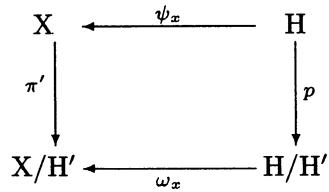
\includegraphics[keepaspectratio]{images/part001_c0ba5876.jpg}}

映射 \((x,\xi)\mapsto\pi'(x\xi)\) 从 \(X\times H\) 到 \(X/H'\) 连续；由于 \(\pi'(x\xi)=\pi'(x\xi\xi')\) 对所有 \(\xi'\in H'\) 成立，该映射通过取商定义了从 \(X\times(H/H')\) 到 \(X/H'\) 的连续映射；因此，对于 X 中每个固定的 x，通过取商得到偏映射 \(\omega_{x}\)，从 \(H/H'\) 到 \(X/H'\)，它由 H 到 X 的映射 \(\psi_x: \xi \mapsto x\xi\) 导出。注意 \(\psi_{x\xi} = \psi_x \circ \gamma_H(\xi)\)，因而 \(\omega_{x\xi} = \omega_x \circ \gamma_{\mathrm{H/H'}}(\xi)\)，对所有 \(\xi \in \mathrm{H}\) 成立。

引理 7. --- 设 K 是 X/H' 的紧子集，L 是 X 的紧子集。则 \(\bigcup_{x\in\mathbf{L}}\omega_{x}^{-1}(\mathbf{K})\) 在 H/H' 中相对紧。

取 \(\mathbf{K}_1\) 为 \(\mathbf{X}\) 的紧子集，满足 \(\pi'(\mathbf{K}_1) = \mathbf{K}\)。令 \(\mathbf{K}_2\) 为 \(\xi \in \mathbf{H}\) 使得 \(\mathbf{L}\xi\) 与 \(\mathbf{K}_1\) 相交的点集。则 \(\mathbf{K}_2\) 是紧的（GT, III, §4, No.~5, Th. 1）。设 \(\xi \in \mathbf{H}\) 满足 \(p(\xi) \in \bigcup_{x \in \mathbf{L}} \omega_x^{-1}(\mathbf{K})\)。于是存在 \(x \in \mathbf{L}\)，使得 \(\omega_x(p(\xi)) \in \mathbf{K}\)，换言之，使得 \(\pi'(x\xi) \in \mathbf{K}\)。由于 \(\pi'(\mathbf{K}_1) = \mathbf{K}\)，存在 \(\xi' \in \mathbf{H}'\)，使得 \(x\xi\xi' \in \mathbf{K}_1\)。于是 \(\xi\xi' \in \mathbf{K}_2\)，因此 \(p(\xi) = p(\xi\xi') \in p(\mathbf{K}_2)\)。由此得到 \(\bigcup_{x \in \mathbf{L}} \omega_x^{-1}(\mathbf{K}) \subset p(\mathbf{K}_2)\)。

这个引理首先表明映射 \(\omega_x\) 是 逆紧的。因此可得到测度 \(\omega_x(\beta/\beta')\)，定义在 \(\mathbf{X}/\mathbf{H}'\) 上，它集中于 \(\omega_x(\mathbf{H}/\mathbf{H}') = \pi'(\psi_x(\mathbf{H})) = \pi'(x\mathbf{H})\)。若 \(f \in \mathcal{K}(\mathbf{X}/\mathbf{H}')\)，则引理 7 和 §1, No.~1, 引理 1 表明，函数 \(x \mapsto \langle f, \omega_x(\beta/\beta') \rangle\) 在 \(\mathbf{X}\) 上连续；此外，\(\langle f, \omega_x(\beta/\beta') \rangle\) 当 \(\operatorname{Supp} f\) 与 \(\pi'(x\mathbf{H})\) 不相交时为零，换言之，当 \(\pi(x)\) 不属于 \(\operatorname{Supp} f\) 在 \(\mathbf{X}/\mathbf{H}\) 中的典范像时，该值为零。

此外，若 \(x \in H\)，则

\[
\omega_ {x \xi} (\beta / \beta^ {\prime}) = \omega_ {x} \left(\boldsymbol {\gamma} _ {\mathrm{H} / \mathrm{H} ^ {\prime}} (\xi) (\beta / \beta^ {\prime})\right) = \omega_ {x} (\beta / \beta^ {\prime}).
\]

因此，映射 \(x \mapsto \omega_x(\beta/\beta')\) 从 X 到 \(\mathcal{M}(\mathrm{X}/\mathrm{H}')\)，通过取商定义了映射 \(u \mapsto (\beta/\beta')_u\) 从 X/H 到 \(\mathcal{M}(\mathrm{X}/\mathrm{H}')\)。上述结果表明，对于每个 \(f \in \mathcal{K}(\mathrm{X}/\mathrm{H}')\)，映射 \(u \mapsto \langle f, (\beta/\beta')_u \rangle\) 连续且具有紧支集。因此，映射 \(u \mapsto (\beta/\beta')_u\) 是一个 \((\mu/\beta)\)-适合的弱连续测度族，取值于 \(\mathrm{X}/\mathrm{H}'\) 上，并以 \(\mathrm{X}/\mathrm{H}\) 为指标集。

设 \(x \in X\)，且 \(u = \pi(x) \in X/H\)。设 \(f\) 是 \(X/H'\) 上取值于 Banach 空间或 \(\overline{R}\) 的函数。由 Ch. V, §4, Th. 2，对于 \(f\) 而言，为 \((\beta/\beta')_u\)-可积的充要条件是，函数 \(p(\xi) \mapsto f\big(\omega_x(p(\xi))\big) = f\big(\pi'(x\xi)\big)\) 在 \(H/H'\) 上为 \((\beta/\beta')\)-可积；在此情形下

\[
\int_ {\mathrm{X} / \mathrm{H} ^ {\prime}} \mathbf {f} (u ^ {\prime}) d (\beta / \beta^ {\prime}) _ {u} (u ^ {\prime}) = \int_ {\mathrm{H} / \mathrm{H} ^ {\prime}} \mathbf {f} \left(\pi^ {\prime} (x \xi)\right) d (\beta / \beta^ {\prime}) (\dot {\xi}) \quad \left(\dot {\xi} = p (\xi)\right).\tag{21}
\]

关于可测性、上积分和本质积分也有相应的性质。

命题 12. --- 在上述记号下，

\[
\int_ {\mathrm{X/H}} (\beta / \beta^ {\prime}) _ {u} d (\mu / \beta) (u) = \mu / \beta^ {\prime}.\tag{22}
\]

设 \(f \in \mathcal{K}(X)\)，并令 \(f^{\flat} \in \mathcal{K}(X/H')\) 由下式定义：

\[
f ^ {\flat} \left(\pi^ {\prime} (x)\right) = \int_ {\mathrm{H} ^ {\prime}} f \left(x \xi^ {\prime}\right) d \beta^ {\prime} \left(\xi^ {\prime}\right).
\]

只需（参见 No.~2）证明 \(f^{\flat}\) 关于 (22) 的两个成员具有相同的积分。现在，\(\langle \mu / \beta', f^{\flat} \rangle = \langle \mu, f \rangle\)。另一方面，

\[
\left\langle \int_ {\mathrm{X} / \mathrm{H}} \left(\beta / \beta^ {\prime}\right) _ {u} d (\mu / \beta) (u), f ^ {\flat} \right\rangle = \int_ {\mathrm{X} / \mathrm{H}} \left\langle \left(\beta / \beta^ {\prime}\right) _ {u}, f ^ {\flat} \right\rangle d (\mu / \beta) (u).
\]

现在取 \(x \in \mathbf{X}\)，并令 \(u = \pi(x)\)。有

\[
\begin{array}{r l} \langle (\beta / \beta^ {\prime}) _ {u}, f ^ {b} \rangle & = \langle \omega_ {x} (\beta / \beta^ {\prime}), f ^ {b} \rangle = \int_ {\mathrm{H/H} ^ {\prime}} f ^ {b} \big (\omega_ {x} (\dot {\xi}) \big) d (\beta / \beta^ {\prime}) (\dot {\xi}) \\ & = \int_ {\mathrm{H/H} ^ {\prime}} f ^ {b} \big (\pi^ {\prime} (x \xi) \big) d (\beta / \beta^ {\prime}) (\dot {\xi}) \\ & = \int_ {\mathrm{H/H} ^ {\prime}} d (\beta / \beta^ {\prime}) (\dot {\xi}) \int_ {\mathrm{H} ^ {\prime}} f (x \xi \xi^ {\prime}) d \beta^ {\prime} (\xi^ {\prime}) \\ & = \int_ {\mathrm{H}} f (x \xi) d \beta (\xi). \end{array}
\]

因此

\[
\left\langle \int_ {\mathrm{X/H}} (\beta / \beta^ {\prime}) _ {u} d (\mu / \beta) (u), f ^ {\flat} \right\rangle = \int_ {\mathrm{X/H}} d (\mu / \beta) (u) \int_ {\mathrm{H}} f (x \xi) d \beta (\xi) = \left\langle \mu , f \right\rangle ,
\]

命题得证。

推论 1. --- a) 设 f 是 X/H' 上取值于 Banach 空间或 \(\overline{\mathbf{R}}\) 的函数，并且关于 \(\mu/\beta'\) 可积。存在 X/H 的一个 \((\mu/\beta)\)-可忽略子集 N，具有如下性质：若 \(x \in X\) 满足 \(\pi(x) \notin N\)，则 H/H' 上的函数 \(\mathbf{f} \circ \omega_x\)，即函数 \(\dot{\xi} \mapsto \mathbf{f}\big(\pi'(x\xi)\big)\)，关于 \(\beta/\beta'\) 可积。积分 \(\int_{H/H'} \mathbf{f}\big(\pi'(x\xi)\big)d(\beta/\beta')(\dot{\xi})\) 只依赖于 \(\dot{x} = \pi(x)\)，并且是一个 \((\mu/\beta)\)-可积函数，关于 \(\dot{x}\)；并且

\[
\int_ {\mathrm{X} / \mathrm{H} ^ {\prime}} \mathbf {f} d (\mu / \beta^ {\prime}) = \int_ {\mathrm{X} / \mathrm{H}} d (\mu / \beta) (\dot {x}) \int_ {\mathrm{H} / \mathrm{H} ^ {\prime}} \mathbf {f} \left(\pi^ {\prime} (x \xi)\right) d (\beta / \beta^ {\prime}) (\dot {\xi}).
\]

\begin{enumerate}
\def\labelenumi{\alph{enumi})}
\setcounter{enumi}{1}
\tightlist
\item
  设 \(f\) 是一个 \(\geqslant 0\) 的函数，定义在 \(\mathbf{X} / \mathbf{H}'\) 上，关于 \(\mu / \beta'\) 可测，并且在某个 \((\mu / \beta')\)-可积集的可数并之外为零。则
\end{enumerate}

\[
\pi (x) \mapsto \int_ {\mathrm{H} / \mathrm{H} ^ {\prime}} ^ {*} f (\pi^ {\prime} (x \xi)) d (\beta / \beta^ {\prime}) (\dot {\xi})
\]

是 \((\mu /\beta)\)-可测的，并且

\[
\int_ {\mathrm {X/ H^ {\prime}}} ^ {*} f d (\mu / \beta^ {\prime}) = \int_ {\mathrm{X/H}} ^ {*} d (\mu / \beta) (\dot {x}) \int_ {\mathrm {H/ H^ {\prime}}} ^ {*} f \bigl (\pi^ {\prime} (x \xi) \bigr) d (\beta / \beta^ {\prime}) (\dot {\xi}).
\]

\begin{enumerate}
\def\labelenumi{\alph{enumi})}
\setcounter{enumi}{2}
\tightlist
\item
  设 f 是 X/H' 上取值于 Banach 空间或 \(\overline{R}\) 的函数，关于 \(\mu/\beta'\) 可测，并且在某个 \((\mu/\beta')\)-可积集的可数并之外为零。则 f 为 \((\mu/\beta')\)-可积的一个充分条件是
\end{enumerate}

\[
\int_ {\mathrm{X} / \mathrm{H}} ^ {*} d (\mu / \beta) (\dot {x}) \int_ {\mathrm{H} / \mathrm{H} ^ {\prime}} ^ {*} | \mathbf {f} (\pi^ {\prime} (x \xi)) | d (\beta / \beta^ {\prime}) (\dot {\xi}) <   + \infty .
\]

推论 2. --- 设 G 是局部紧群，A、B 是 G 的满足 A ⊃ B 的闭子群。假设关于 B 的左陪集齐性空间 G/B 上存在关于 G 不变且有界的非零正测度 α。

\begin{enumerate}
\def\labelenumi{\alph{enumi})}
\item
  \(\alpha\) 在 \(\mathbf{G} / \mathbf{A}\) 中的典范像是关于 \(\mathbf{G}\) 不变且有界的非零正测度。
\item
  \(\Delta_{\mathrm{G}}\) 在 A 上与 \(\Delta_{\mathrm{A}}\) 一致，在 B 上与 \(\Delta_{\mathrm{B}}\) 一致。
\item
  关于 B 的 A 的左陪集齐性空间 A/B 上存在关于 A 不变且有界的非零正测度。
\end{enumerate}

断言 a) 显然。断言 b) 由 a) 和 No.~6, Th. 3 的 Cor. 2 得出。由 b)，\(\Delta_{\mathbf{A}}\) 在 B 上与 \(\Delta_{\mathbf{B}}\) 一致，因而可将本小节的结果应用于 \(\mathbf{X} = \mathbf{G}\)、\(\mathbf{H} = \mathbf{A}\)、\(\mathbf{H}' = \mathbf{B}\) 的情形。\(\mathbf{G} / \mathbf{B}\) 上恒等于 1 的函数关于 \(\alpha\) 可积。由推论 1 的 a)，\(\mathbf{A} / \mathbf{B}\) 上恒等于 1 的函数关于 \(\beta / \beta'\) 可积，其中 \(\beta\) 和 \(\beta'\) 分别表示 A 和 B 上的左 Haar 测度；因此 \(\beta / \beta'\) 有界。

\subsection{由某些子群的 Haar 测度构造群的 Haar 测度}

设 \(\mathbf{G}\) 是局部紧群，\(\mathbf{X}\) 和 \(\mathbf{Y}\) 是 \(\mathbf{G}\) 的两个闭子群，且 \(\Omega = \mathbf{XY}\) 包含一个邻域 \(\mathbf{U}\)，其中包含 \(e\)。则 \(\Omega\) 是 \(\mathbf{G}\) 中的开集；事实上，对于任意 \(x_0 \in \mathbf{X}\) 和 \(y_0 \in \mathbf{Y}\)，有 \(\mathbf{XY} = (x_0\mathbf{X})(\mathbf{Y}y_0) \supset x_0\mathbf{U}y_0\)，而 \(x_{0}Uy_{0}\) 是 \(x_{0}y_{0}\) 的邻域；因此 \(\Omega\) 是其每一点的邻域。

*当 G 是李群且其李代数为 g 时，如果 X、Y 所对应的子代数之和为 g，则关于 X、Y 的条件得到满足。*

群 \(X \times Y\) 按作用律 \((x, y) \cdot s = xsy^{-1}\)（\(x \in X, y \in Y, s \in G\)）在 G 上连续地从左作用。令 \(Z = X \cap Y\)。\(X \times Y\) 中 e 的稳定子是子群 \(Z_{0}\)（它属于 \(X \times Y\)），它由 \((z, z)\)（其中 \(z \in Z\)）这些对组成，并且是与 Z 典范同构的子群。因此，集合 \(\Omega\) 可识别为左陪集齐性空间 \((X \times Y)/Z_{0}\)；更准确地说，映射 \((x, y) \mapsto xy^{-1}\) 从 \(X \times Y\) 到 \(\Omega\)，通过取商定义了从 \((X \times Y)/Z_{0}\) 到 \(\Omega\) 的连续双射。我们假设该映射是同胚。（当 G 在无穷远处可数时尤其如此：参见 App. I。）

命题 13. --- 进一步假设 Z 是紧的。设 \(\mu_{\mathrm{G}}\)、\(\mu_{\mathrm{X}}\)、\(\mu_{\mathrm{Y}}\) 分别是 G、X、Y 上的左 Haar 测度，\(\Lambda\) 是 \(\Delta_{\mathrm{G}}\) 在 Y 上的限制。则限制 \(\mu\)（即 \(\mu_{\mathrm{G}}\) 在 \(\Omega\) 上的限制），除一个常数因子外，是 \(\mu_{\mathrm{X}} \otimes (\Lambda^{-1} \cdot \mu_{\mathrm{Y}})\) 在映射 \((x, y) \mapsto xy^{-1}\) 从 X × Y 到 \(\Omega\) 下的像（该映射是 逆紧的）。

对于 \(x\in \mathbf{X},y\in \mathbf{Y}\)，

\[
\boldsymbol {\gamma} \big ((x, y) \big) \mu = \boldsymbol {\delta} (y) \boldsymbol {\gamma} (x) \mu = \Delta_ {G} (y) \mu .
\]

将 \(\Omega\) 与齐性空间 \((\mathrm{X} \times \mathrm{Y}) / \mathrm{Z}_0\) 识别，并在 \(\mathbf{Z}_0\) 上选取适当的 Haar 测度，可见 \(\mu^\sharp\) 是 \(\mathrm{X} \times \mathrm{Y}\) 的左 Haar 测度（即 \(\mu_{\mathrm{X}} \otimes \mu_{\mathrm{Y}}\)）乘以函数 \((x, y) \mapsto \Delta_{\mathrm{G}}(y)^{-1}\) 所得的测度（No.~6, 引理 6）。另一方面，\(\mu\) 除一个常数因子外，是 \(\mu^\sharp\) 在从 \(\mathrm{X} \times \mathrm{Y}\) 到 \(\Omega\) 的典范映射下的像（No.~3, 注记 2）。

推论。--- 设 f 是定义在 \(\Omega\) 上、取值于 Banach 空间或 \(\overline{R}\) 的函数。f 关于 \(\mu\) 可积的充要条件是，函数 \((x,y)\mapsto\mathbf{f}(xy)\Delta_{\mathrm{G}}(y)\Delta_{\mathrm{Y}}(y)^{-1}\) 关于 \((\mu_{\mathrm{X}}\otimes\mu_{\mathrm{Y}})\) 可积；在此情形下

\[
\int_ {\Omega} \mathbf {f} (\omega) d \mu (\omega) = a \iint_ {\mathrm{X} \times \mathrm{Y}} \mathbf {f} (x y) \Delta_ {\mathrm{G}} (y) \Delta_ {\mathrm{Y}} (y) ^ {- 1} d \mu_ {\mathrm{X}} (x) d \mu_ {\mathrm{Y}} (y),\tag{23}
\]

其中 \(a\) 是一个 \(>0\) 且与 \(\mathbf{f}\) 无关的常数。

由 Prop. 13 和 Ch. V, §4, No.~4, Th. 2，f 关于 \(\mu\) 可积的充要条件是，函数 \((x,y)\mapsto\mathbf{f}(xy^{-1})\) 关于 \(\mu_{\mathrm{X}}\otimes(\Lambda^{-1}\cdot\mu_{\mathrm{Y}})\) 可积；或者等价地，函数 \((x,y)\mapsto\mathbf{f}(xy^{-1})\Delta_{\mathrm{G}}(y)^{-1}\) 关于 \(\mu_{X}\otimes\mu_{Y}\) 可积；或者等价地，函数 \((x,y)\mapsto\mathbf{f}(xy)\Delta_{\mathrm{G}}(y)\Delta_{\mathrm{Y}}(y)^{-1}\) 关于 \(\mu_{X}\otimes\mu_{Y}\) 可积。公式 (23) 由类似论证得出。

命题 14. --- 假设 Prop. 13 的条件成立，并且进一步假设 Y 是正规的。

\begin{enumerate}
\def\labelenumi{\alph{enumi})}
\item
  \(\mu_{\mathrm{G}}\) 在 \(\Omega\) 上的限制，除一个常数因子外，是 \(\mu_{\mathrm{X}} \otimes \mu_{\mathrm{Y}}\) 在映射 \((x,y) \mapsto xy\) 从 \(\mathrm{X} \times \mathrm{Y}\) 到 \(\Omega\) 下的像。
\item
  对于 \(x \in \mathbf{X}\) 和 \(y \in \mathbf{Y}\)，
\end{enumerate}

\[
\Delta_ {\mathrm{G}} (x y) = \Delta_ {\mathrm{X}} (x) \Delta_ {\mathrm{Y}} (y) \bmod (i _ {x}),
\]

其中 \(i_x\) 表示 Y 的自同构 \(v \mapsto x^{-1}vx\)。

由 Prop. 10 b)，\(\Delta_{\mathrm{G}} = \Delta_{\mathrm{Y}}\) 在 Y 上成立，因此 a) 由 (23) 得出。取 \(x_0 \in \mathbf{X}\)、\(y_0 \in \mathbf{Y}\)。记 \(p\) 为映射 \((x, y) \mapsto xy\)，从 \(\mathbf{X} \times \mathbf{Y}\) 到 \(\Omega\)。由于

\[
x y \left(x _ {0} y _ {0}\right) ^ {- 1} = x x _ {0} ^ {- 1} \left(x _ {0} y y _ {0} ^ {- 1} x _ {0} ^ {- 1}\right) = x x _ {0} ^ {- 1} i _ {x _ {0} ^ {- 1}} \left(y y _ {0} ^ {- 1}\right),
\]

我们有

\[
\begin{array}{r l} \Delta_ {\mathrm{G}} (x _ {0} y _ {0}) p (\mu_ {\mathrm{X}} \otimes \mu_ {\mathrm{Y}}) & = \pmb {\delta} (x _ {0} y _ {0}) p (\mu_ {\mathrm{X}} \otimes \mu_ {\mathrm{Y}}) \\ & = p \big (\pmb {\delta} (x _ {0}) \mu_ {\mathrm{X}} \otimes i _ {x _ {0} ^ {- 1}} \pmb {\delta} (y _ {0}) \mu_ {\mathrm{Y}} \big) \\ & = p \big (\Delta_ {\mathrm{X}} (x _ {0}) \mu_ {\mathrm{X}} \otimes \Delta_ {\mathrm{Y}} (y _ {0}) (\bmod i _ {x _ {0}}) \mu_ {\mathrm{Y}} \big) \\ & = \Delta_ {\mathrm{X}} (x _ {0}) \Delta_ {\mathrm{Y}} (y _ {0}) (\bmod i _ {x _ {0}}) p (\mu_ {\mathrm{X}} \otimes \mu_ {\mathrm{Y}}), \end{array}
\]

从而得到 b)。

注记。--- 当 G 是 X 与 Y 的拓扑半直积时，Prop. 14 特别适用（GT, III, §2, No.~10）。此时 \(Z = \{e\}\) 且 \(\Omega = G\)。由于有 \(yx = x i_{x}(y)\)，对 \(x \in X\)、\(y \in Y\) 成立，测度 \(\mu_{G}\) 也等于 \((\text{mod } i_{x})\mu_{X} \otimes \mu_{Y}\) 在映射 \((x, y) \mapsto yx\) 从 \(X \times Y\) 到 G 下的像，差一个常数因子。

\subsection{基本域上的积分}

设 X 是局部紧空间，H 是在 X 上连续且 逆紧地从右作用的离散群。令 \(\pi\) 为从 X 到 X/H 的典范映射。对于每个 \(x \in X\)，记 H 中 x 的稳定子为 \(H_x\)；这是 H 的有限子群（GT, III, §4, No.~2, Prop. 4）；其阶记为 \(n(x)\)。对于每个 \(s \in H\)，有 \(H_{xs} = s^{-1}H_x s\)，因而 \(n(xs) = n(x)\)。存在 x 的开邻域 U，使得 \(U \cap Us = \varnothing\) 对 \(s \notin H_x\) 成立（同上, No.~4, Prop. 8 的证明）；对于 \(y \in U\)，有 \(H_y \subset H_x\)；因此 X 上的函数 n 是上半连续的。当 X 在无穷远处可数时，H 可数；事实上，设 \((\mathrm{K}_1, \mathrm{K}_2, \ldots)\) 是由紧子集序列覆盖 X 的覆盖，并取 \(x_{0} \in X\)；\(s \in H\) 满足 \(x_{0}s \in K_{i}\) 的这些元素所成的集合是有限的（同上, No.~5, Th. 1），从而得到所述结论。

定义 2. --- 设 \(F \subset X\)。如果 \(\pi\) 在 F 上的限制是从 F 到 X/H 的双射（换言之，F 是 H 所定义的等价关系的代表元系），则称 F 为（关于 H 的）基本域。

引理 8. --- 设 F 是基本域。对于每个 \(x \in \mathbf{X}\)，

\[
\sum_ {s \in \mathrm{H}} \varphi_ {\mathrm{F} s} (x) = n (x).\tag{24}
\]

由于有 \(\varphi_{\mathrm{Fs}}(xt) = \varphi_{\mathrm{Fst}^{-1}}(x)\)，对所有 \(s\) 和 \(t\) 属于 \(\mathbf{H}\) 成立，当 \(x\) 替换为 \(xt\) 时，(24) 的两边仍保持不变。因此可设 \(x \in \mathbf{F}\)。此时有以下等价关系

\[
\varphi_ {\mathrm{Fs}} (x) = 1 \Leftrightarrow x \in \mathrm{Fs} \Leftrightarrow x s ^ {- 1} \in \mathrm{F} \Leftrightarrow x s ^ {- 1} = x \Leftrightarrow s \in \mathrm{H} _ {x},
\]

从而得到 (24)。

命题 15. --- 假设 X 在无穷远处可数。设 \(\mu\) 是 X 上的 \(\geqslant 0\) 测度。设 F 是基本域，并且 Fs 都是 \(\mu\)-可测的，对每个 \(s \in H\) 成立。设 f 是一个 \(\mu\)-可积函数，定义在 X 上，取值于 Banach 空间或 \(\overline{\mathbf{R}}\)。则族

\[
\int_ {\mathrm{Fs}} n (x) ^ {- 1} \mathbf {f} (x) d \mu (x) \quad (s \in \mathbf {H})
\]

是可求和的，并且

\[
\int_ {\mathrm{X}} \mathbf {f} (x) d \mu (x) = \sum_ {s \in \mathrm{H}} \int_ {\mathrm{F} s} n (x) ^ {- 1} \mathbf {f} (x) d \mu (x).
\]

若 \(\mathbf{A}\) 是 \(\mathbf{H}\) 的有限子集，则

\[
\left| \sum_ {s \in \mathrm{A}} n ^ {- 1} \mathbf {f} \varphi_ {\mathrm{Fs}} \right| \leqslant n ^ {- 1} | \mathbf {f} | \sum_ {s \in \mathrm{A}} \varphi_ {\mathrm{Fs}} \leqslant | \mathbf {f} |
\]

由引理 8 得出。引理 8 还证明，\(\sum_{s\in\mathbf{A}}n^{-1}\mathbf{f}\varphi_{\mathrm{F}s}\) 逐点收敛到 \(\mathbf{f}\)，其中指标集是由 \(\mathbf{H}\) 的有限子集构成的递增有向集。于是 Prop. 15 由 Ch. IV, §4, No.~3, Th. 2 得出。

定理 4. --- 设 X 是在无穷远处可数的局部紧空间，H 是在 X 上连续且 逆紧地从右作用的离散群，\(\pi\) 是从 X 到 X/H 的典范映射，\(\mu\) 是 X 上关于 H 不变的正测度，\(\beta\) 是 H 的归一化 Haar 测度，且 \(\lambda = \mu/\beta\)。设 F 是 \(\mu\)-可测的基本域。

\begin{enumerate}
\def\labelenumi{\alph{enumi})}
\tightlist
\item
  偶 \((\pi, n^{-1}\varphi_{\mathrm{F}})\) 对 \(\mu\) 是适合的，并且
\end{enumerate}

\[
\int_ {\mathrm{X}} n (x) ^ {- 1} \varphi_ {\mathrm{F}} (x) \varepsilon_ {\pi (x)} d \mu (x) = \lambda .
\]

\begin{enumerate}
\def\labelenumi{\alph{enumi})}
\setcounter{enumi}{1}
\item
  映射 \(\pi\) 关于 \(n^{-1}\varphi_{\mathrm{F}}\cdot \mu\) 是 逆紧的，并且 \(\pi (n^{-1}\varphi_{\mathrm{F}}\cdot \mu) = \lambda\)。
\item
  设 k 是 X/H 上的函数。k 关于 \(\lambda\) 可测（分别为 \(\lambda\)-可积）的充要条件是 \(n^{-1}\varphi_{\mathrm{F}}(k\circ\pi)\) 关于 \(\mu\) 可测（分别为 \(\mu\)-可积）；并且，若 k 关于 \(\lambda\) 可积，则
\end{enumerate}

\[
\int_ {\mathrm{X/H}} k d \lambda = \int_ {\mathrm{F}} n ^ {- 1} (k \circ \pi) d \mu .
\]

我们有 \(\mu = \lambda^{\sharp}\)。设 \(f \in \mathcal{H}_{+}(\mathrm{X / H})\)。则 \(n^{-1}\varphi_{\mathrm{F}}(f \circ \pi)\) 关于 \(\mu\) 可测且 \(\geqslant 0\)，由 No.~3 的 Prop. 5 b) 有

\[
\int_ {\mathrm{X}} ^ {*} n (x) ^ {- 1} \varphi_ {\mathrm{F}} (x) f (\pi (x)) d \mu (x) = \int_ {\mathrm{X/H}} ^ {*} f (\dot {x}) d \lambda (\dot {x}) \int_ {\mathrm{H}} ^ {*} n (x \xi) ^ {- 1} \varphi_ {\mathrm{F}} (x \xi) d \beta (\xi)
\]

并且由引理 8，\(\int_{\mathrm{H}}^{*}n(x\xi)^{-1}\varphi_{\mathrm{F}}(x\xi)d\beta (\xi) = n(x)^{-1}\sum_{\xi \in \mathrm{H}}\varphi_{\mathrm{F}}(x\xi) = 1\)。因此 \(n^{-1}\varphi_{\mathrm{F}}\cdot (f\circ \pi)\) 关于 \(\mu\) 可积，并且

\[
\int_ {\mathrm{X}} n (x) ^ {- 1} \varphi_ {\mathrm{F}} (x) f (\pi (x)) d \mu (x) = \int_ {\mathrm{X/H}} f (\dot {x}) d \lambda (\dot {x}).
\]

这证明了 a)。b) 的断言类似可证。c) 的断言可由 a) 以及 Ch. V, §4, Prop. 3 和 Th. 2 得出。

推论。--- 保持 Th. 4 的假设和记号。设 F' 是第二个 μ-可测基本域。设 u 是 X 上取值于 Banach 空间或 \(\overline{R}\) 的函数，并且关于 H 不变。假设 u 在 F 上 μ-可积。则 u 在 F' 上 μ-可积，并且

\[
\int_ {\mathrm{F}} \mathbf {u} (x) d \mu (x) = \int_ {\mathrm{F} ^ {\prime}} \mathbf {u} (x) d \mu (x).
\]

由于 \(\mathbf{u}\) 和 \(n\) 关于 \(\mathbf{H}\) 不变，存在函数 \(\mathbf{v}\)，定义在 \(\mathrm{X / H}\) 上，使得 \(\mathbf{v} \circ \pi\) 与 \(n\mathbf{u}\) 在 \(\mathbf{F}\) 和 \(\mathbf{F}'\) 上一致。于是 \(n^{-1}\varphi_{\mathrm{F}}(\mathbf{v}\circ \pi) = \varphi_{\mathrm{F}}\mathbf{u}, n^{-1}\varphi_{\mathrm{F}^{\prime}}(\mathbf{v}\circ \pi) = \varphi_{\mathrm{F}^{\prime}}\mathbf{u}.\) 根据假设，\(n^{-1}\varphi_{\mathrm{F}}(\mathbf{v}\circ \pi)\) 关于 \(\mu\) 可积。由 Th. 4，\(\mathbf{v}\) 关于 \(\lambda\) 可积，\(\varphi_{\mathrm{F}^{\prime}}\mu\) 关于 \(\mu\) 可积，并且

\[
\int_ {\mathrm{F}} \mathbf {u} d \mu = \int_ {\mathrm{X/H}} \mathbf {v} d \lambda = \int_ {\mathrm{F} ^ {\prime}} \mathbf {u} d \mu .
\]

关于 \(\mu\)-可测基本域的存在性，见 Exer. 12。

\section{应用和例子}

\subsection{线性映射的紧群}

设 E 是 R、C 或 H 上的有限维向量空间。则 End(E) 是 R 上的有限维代数，而 End(E) 上的典范拓扑（§1, No.~10）就是紧收敛拓扑。群 \(\operatorname{Aut}(E) = \mathbf{GL}(E)\) 是 End(E) 的开子集，因而是局部紧群。设 \((e_{1}, e_{2}, \ldots, e_{n})\) 是 E 的一组基，对于 E 的每个自同态 u，令 \(M(u) = (\alpha_{ij}(u))\) 为 u 关于此基的矩阵；End(E) 的子集 S 在 End(E) 中相对紧，等价于函数 \(\alpha_{ij}(u)\) 在 S 上有界。

命题 1. --- 设 G 是 Aut(E) 的子群。以下三个性质等价：

\begin{enumerate}
\def\labelenumi{(\roman{enumi})}
\item
  G 在 \(\operatorname{End}(\mathbf{E})\) 中相对紧；
\item
  G 在 \(\operatorname{Aut}(\mathbf{E})\) 中相对紧；
\item
  G 保持 E 上的一个非退化 \(^{1}\) 正厄米形式不变。(iii) \(\Rightarrow\) (i)：假设 G 保持非退化正厄米形式 \(\Psi\) 不变。取 \((e_{1},\ldots,e_{n})\) 为 \(\Psi\) 的一组标准正交基（Alg., Ch. IX, §6, No.~1, Cor. 1 of Th. 1）。对于每个 \(u\in G\)，令 \((u_{ij})\) 为 u 关于 \((e_{i})\) 的矩阵。对于任意 j，有 \(\sum_{i=1}^{n}|u_{ij}|^{2}=1\)，故对于所有 i 和 j 都有 \(|u_{ij}|\leqslant1\)，这就证明了 (i)。
\item
  \(\Rightarrow\) (ii)：这由 GT, X, §3, No.~5, Th. 4 的 Cor. 得出，同时注意到 \(\operatorname{End}(\mathbf{E})\) 的拓扑是紧收敛拓扑。
\item
  \(\Rightarrow\) (iii)：假设 \(\overline{\mathbf{G}}\) 是 \(\mathbf{G}\) 在 \(\operatorname{Aut}(\mathbf{E})\) 中的闭包且是紧的。设 \(\Phi\) 是 \(\mathbf{E}\) 上的非退化正厄米形式。若标量域是 \(\mathbf{R}\) 或 \(\mathbf{C}\)，则由 \(\Phi\) 使 \(\mathbf{E}\) 成为有限维 Hilbert 空间，性质 (iii) 将由下述引理得到：
\end{enumerate}

引理 1. --- 设 F 是 Hilbert 空间，K 是紧群，且 \(s \mapsto U(s)\) 是 K 到 \(\mathcal{L}(\mathrm{F};\mathrm{F})\) 的可逆元群中的表示，并且关于逐点收敛拓扑连续。则 F 上存在非退化正厄米形式 \(\varphi\)，使得

\[
\varphi (U (s) x, U (s) y) = \varphi (x, y)
\]

对于所有 \(s \in \mathbf{K}\)、\(x \in \mathbf{F}\) 和 \(y \in \mathbf{F}\) 成立，并且 \(\mathbf{F}\) 上由 \(\varphi\) 定义的拓扑向量空间结构（TVS, V, §1, No.~3）与 \(\mathbf{F}\) 的原有结构相同。

设 \(\alpha\) 是 \(\mathbf{K}\) 上的 Haar 测度。对于任意 \(x, y\)，在 \(\mathbf{F}\) 中，映射 \(s \mapsto (U(s)x|U(s)y)\) 连续。置

\[
\varphi (x, y) = \int (U (s) x | U (s) y) d \alpha (s).
\]

显然，\(\varphi(x,y)\) 是 \(\mathbf{F}\) 上的半双线性形式。由于自同态集 \(U(s)\) 在 \(\mathcal{L}_s(\mathrm{F};\mathrm{F})\) 中紧，存在常数 \(\mathbf{M}\)，使得 \(\| U(s)\| \leqslant \mathbf{M}\) 对所有 \(s\in \mathbf{K}\) 成立。因此对于每个 \(x\in \mathbf{F}\)，有

\[
\mathrm{M} ^ {- 1} \| x \| \leqslant \| U (s) x \| \leqslant \mathrm{M} \| x \|,
\]

从而有不等式

\[
\mathbf {M} ^ {- 2} \alpha (\mathbf {K}) \| x \| ^ {2} \leqslant \varphi (x, x) \leqslant \mathbf {M} ^ {2} \alpha (\mathbf {K}) \| x \| ^ {2},
\]

这表明 \(\varphi\) 是正且非退化的，并且范数 \(\varphi(x,x)^{1/2}\) 与范数 \(\|x\|\) 等价。最后，对于所有 \(t \in K\)，

\[
\begin{array}{r l} & {\varphi (U (t) x, U (t) y) = \int (U (s t) x | U (s t) y) d \alpha (s)} \\ & {\qquad = \int (U (s) x | U (s) y) d \alpha (s) = \varphi (x, y).} \end{array}
\]

当标量域为 H 时，只需完全类似地处处将函数 \(s \mapsto (U(s)x|U(s)y)\) 换成定义在 G 上、取值于 H 的函数 \(s \mapsto \Phi(sx, sy)\)。命题得证。

注记。--- 设 \(\Phi\) 是 E 上的非退化正厄米形式。酉群 \(\mathbf{U}(\Phi)\) 在 \(\operatorname{Aut}(\mathbf{E})\) 中是闭的，因而是紧的（Prop. 1）。Prop. 1 还表明，\(\operatorname{Aut}(\mathbf{E})\) 的每个紧子群都包含于某个形如 \(\mathbf{U}(\Phi)\) 的子群中。现在若 \(\mathbf{U}(\Phi)\) 包含于 \(\operatorname{Aut}(\mathbf{E})\) 的紧子群 K 中，则可见存在 E 上的非退化正厄米形式 \(\Phi'\)，使得 \(\mathbf{U}(\Phi) \subset \mathbf{K} \subset \mathbf{U}(\Phi')\)；并且容易推出（Exer. 1），\(\Phi\) 与 \(\Phi'\) 成比例，从而 \(\mathbf{U}(\Phi) = K\)。因此，\(\operatorname{Aut}(E)\) 的极大紧子群正是形如 \(\mathbf{U}(\Phi)\) 的子群。

\subsection{纤维空间和群扩张的平凡性}

命题 2. --- 设 X 是局部紧空间，局部紧群 H 通过 \((x,\xi)\mapsto x\xi\) 在其中连续且 逆紧地从右作用。假设 X/H 仿紧。设 g 是 H 到 \(R^{n}\) 的连续表示。则存在从 X 到 \(R^{n}\) 的连续映射 f，使得 \(f(x\xi)=f(x)+g(\xi)\) 对所有 \(x\in X\) 和 \(\xi\in H\) 成立。

立即可归结为 n = 1 的情形。由于加法群 R 与乘法群 \(R_{+}^{*}\) 同构，此时命题立即由 §2, No.~4 的 Prop. 7 得出。

推论。--- 设 X 是局部紧空间，一个有限维实向量空间 V 通过 \((x,v)\mapsto xv\) 在其中连续且 逆紧地从右作用。令 \(\pi\) 为从 X 到 B = X/V 的典范映射。假设 B 仿紧。

\begin{enumerate}
\def\labelenumi{\alph{enumi})}
\item
  存在连续映射 \(f\)，定义在 \(\mathbf{X}\) 上取值于 \(\mathbf{V}\)，满足 \(f(xv) = f(x) + v\)，对所有 \(x \in \mathbf{X}\) 和 \(v \in \mathbf{V}\) 成立。
\item
  若 \(f\) 是满足 a) 条件的映射，则映射 \(x \mapsto (\pi(x), f(x))\) 是从 \(X\) 到 \(B \times V\) 的同胚。
\end{enumerate}

断言 a) 由 Prop. 2 得出，其中 g 取为 V 的恒等映射。设 f 是满足 a) 条件的映射。从 X 到 X 的映射 \(x \mapsto x \cdot (-f(x))\) 连续，并且在每个轨道上为常值，因而具有 \(\varphi \circ \pi\) 的形式，其中 \(\varphi\) 是从 B 到 X 的连续映射；对于每个 \(b \in B\)，有 \(\pi(\varphi(b)) = b\)。从 X 到 B × V 的映射 \(x \mapsto (\pi(x), f(x))\) 与从 B × V 到 X 的映射 \((b, v) \mapsto \varphi(b) \cdot v\) 互为逆映射，因为 \(\varphi(\pi(x)) \cdot f(x) = x \cdot (-f(x)) \cdot (f(x)) = x\)、\(\pi(\varphi(b) \cdot v) = \pi(\varphi(b)) = b\)，并且若 \(b = \pi(y)\)，则

\[
f (\varphi (\pi (y)) \cdot v) = f (y \cdot (- f (y)) \cdot v) = f (y) - f (y) + v = v.
\]

由于这些映射连续，它们是同胚。

注记。--- 设 E 是有限维实仿射空间，T 是紧空间，\(\mu\) 是 T 上总质量为 1 的测度，f 是从 T 到 E 的连续映射。若在 E 中选定原点 a，则 E 由此具有向量空间结构，因而积分 \(\int_{\mathrm{T}} f(t) d\mu(t)\) 有意义；它表示 E 中满足下式的点 x：

\[
x - a = \int_ {\mathrm{T}} (f (t) - a) d \mu (t).
\]

这个点与 \(a\) 的选择无关。事实上，设 \(a' \in \mathbf{E}\) 和 \(x' \in \mathbf{E}\) 满足 \(x' - a' = \int_{\mathbf{T}} (f(t) - a') d\mu(t)\)。则

\[
\begin{array}{c} x ^ {\prime} - a = (x ^ {\prime} - a ^ {\prime}) + (a ^ {\prime} - a) = \int_ {\mathrm{T}} \bigl (f (t) - a ^ {\prime} \bigr) d \mu (t) + \int_ {\mathrm{T}} (a ^ {\prime} - a) d \mu (t) \\ = \int_ {\mathrm{T}} \bigl (f (t) - a \bigr) d \mu (t) = x - a, \end{array}
\]

从而 \(x' = x\)。因此，可以使用符号 \(\int_{\mathrm{T}} f(t) d\mu(t)\)，而不必指明 E 中原点的选择。若 u 是从 E 到另一个有限维仿射空间 \(E'\) 的仿射映射，则

\[
u \Big (\int_ {\mathrm{T}} f (t) d \mu (t) \Big) = \int_ {\mathrm{T}} u \big (f (t) \big) d \mu (t).
\]

事实上，可以将 E 和 \(E'\) 以某种方式识别为向量空间，使 u 成为线性映射；此时该公式已知（Ch. III, §3, No.~2, Prop. 2 和 No.~3, Prop. 7）。

引理 2. --- 设 G 是紧群，\(\mu\) 是 G 的归一化 Haar 测度，E 是有限维实仿射空间，A 是 E 的仿射群，\(\rho\) 是从 G 到 A 的同态。假设对于每个 \(x \in \mathbf{E}\)，从 G 到 E 的映射 \(s \mapsto \rho(s)x\) 连续。则对于每个 \(x \in \mathbf{E}\)，点

\[
x _ {0} = \int_ {\mathrm{G}} \rho (s) x d \mu (s) \in \mathrm{E}
\]

在 G 下不变。

事实上，对于每个 \(t \in G\)，

\[
\rho (t) x _ {0} = \int_ {\mathrm{G}} \rho (t) \rho (s) x d \mu (s) = \int_ {\mathrm{G}} \rho (t s) x d \mu (s) = \int_ {\mathrm{G}} \rho (s) x d \mu (s) = x _ {0}.
\]

命题 3. --- 设 G 是局部紧群。设 H 是 G 的闭正规子群，同构于 \(\mathbf{R}^n\)，且 \(\mathbf{G} / \mathbf{H}\) 是紧的。

\begin{enumerate}
\def\labelenumi{\alph{enumi})}
\item
  存在闭子群 \(\mathbf{L}\)，它是 \(\mathbf{G}\) 的闭子群，使得 \(\mathbf{G}\) 是 \(\mathbf{L}\) 与 \(\mathbf{H}\) 的拓扑半直积。
\item
  若 \(\mathbf{M}\) 是 \(\mathbf{G}\) 的紧子群，则存在 \(x \in \mathbf{H}\)，使得 \(x^{-1}\mathbf{M}x \subset \mathbf{L}\)。
\item
  \(\mathbf{G}\) 的每个紧子群都包含于某个极大紧子群中。
\item
  \(\mathbf{G}\) 的极大紧子群正是 \(\mathbf{L}\) 在 \(\mathbf{G}\) 的内自同构下的变换像。
\end{enumerate}

令 \(\pi\) 为从 \(\mathbf{G}\) 到 \(\mathbf{K} = \mathbf{G} / \mathbf{H}\) 的典范同态。通过取商，映射 \((s,h)\mapsto shs^{-1}\) 从 \(\mathbf{G}\times \mathbf{H}\) 到 \(\mathbf{H}\) 定义了连续映射 \((\sigma ,h)\mapsto \sigma \cdot h\) 从 \(\mathbf{K}\times \mathbf{H}\) 到 \(\mathbf{H}\)，使得 \(shs^{-1} = \pi (s)\cdot h\)。我们将 \(\mathbf{H}\) 识别为 \(\mathbf{R}^n\)（因此，对于群 \(\mathbf{H}\) 的运算，视情形使用乘法或加法记号）。由 Prop. 2 的推论，存在连续映射 \(f\)，从 \(\mathbf{G}\) 到 \(\mathbf{H}\)，使得 \(f(xh) = f(x) + h\)，对 \(x\in \mathbf{G}, h\in \mathbf{H}\) 成立。对于每个 \(x\in \mathbf{G}\)，令 \(p(x) = x\cdot (-f(x))\)，它只依赖于 \(x\) 关于 \(\mathbf{H}\) 的陪集。置

\[
\begin{array}{r l} \mathrm{F} (x, y) & = p (x y) ^ {- 1} p (x) p (y) = f (x y) y ^ {- 1} x ^ {- 1} x (- f (x)) y (- f (y)) \\ & = f (x y) [ y ^ {- 1} (- f (x)) y ] (- f (y)) \\ & = f (x y) - \pi (y) ^ {- 1} f (x) - f (y). \end{array}\tag{1}
\]

我们看到，若对于 G 中所有 x,y 都有 \(F(x,y) = 0\)，则 \(p(G) = L\) 是 G 的子群，并且与 H 的每个陪集恰好交于一点。由于 p 连续，G 于是是 L 与 H 的拓扑半直积（GT, III, §2, No.~10）。

现在，对于任意 \(h, h' \in H\)，

\[
\begin{array}{r l} F (x h, y h ^ {\prime}) & = f (x h y h ^ {\prime}) - \pi (y) ^ {- 1} f (x h) - f (y h ^ {\prime}) \\ & = f (x h y) + h ^ {\prime} - \pi (y) ^ {- 1} f (x) - \pi (y) ^ {- 1} h - f (y) - h ^ {\prime} \\ & = f \big (x y (\pi (y) ^ {- 1} h) \big) - \pi (y) ^ {- 1} f (x) - f (y) - \pi (y) ^ {- 1} h \\ & = f (x y) - \pi (y) ^ {- 1} f (x) - f (y) = F (x, y). \end{array}
\]

因此，F 通过取商定义了连续映射 \(\varphi\)，从 \(K \times K\) 到 H。

另一方面，对于任意 \(x, y, z\)，在 \(\mathbf{G}\) 中，有

\[
\begin{array}{r l} & {\mathrm{F} (z, x y) + \mathrm{F} (x, y) = f (z x y) - \pi (x y) ^ {- 1} f (z) - f (x y) + f (x y)} \\ & {\qquad - \pi (y) ^ {- 1} f (x) - f (y)} \\ & {\qquad = \pi (y) ^ {- 1} f (z x) - \pi (x y) ^ {- 1} f (z) - \pi (y) ^ {- 1} f (x) + f (z x y)} \\ & {\qquad - \pi (y) ^ {- 1} f (z x) - f (y)} \\ & {\qquad = \pi (y) ^ {- 1} \mathrm{F} (z, x) + \mathrm{F} (z x, y),} \end{array}
\]

因此，对于任意 \(x', y', z'\)，在 \(\mathbf{K}\) 中，

\[
- \varphi (x ^ {\prime}, y ^ {\prime}) = \varphi (z ^ {\prime}, x ^ {\prime} y ^ {\prime}) - y ^ {- 1} \varphi (z ^ {\prime}, x ^ {\prime}) - \varphi (z ^ {\prime} x ^ {\prime}, y ^ {\prime}).
\]

对 \(z'\) 使用 K 的归一化 Haar 测度 \(\alpha\) 积分。置 \(\psi(x') = \int \varphi(z', x') d\alpha(z')\)，则 \(\psi\) 是 K 上的连续函数，并且（注意到由 GT, VII, §2, No.~1, Prop. 1，K 在 \(R^{n}\) 上的运算保持 \(R^{n}\) 的向量空间结构）得到

\[
- \varphi (x ^ {\prime}, y ^ {\prime}) = \psi (x ^ {\prime} y ^ {\prime}) - y ^ {- 1} \psi (x ^ {\prime}) - \psi (y ^ {\prime}).
\]

换言之，置 \(k - \psi \circ \pi\)，这是 G 上的连续函数，

\[
- \mathrm{F} (x, y) = k (x y) - \pi (y) ^ {- 1} k (x) - k (y).\tag{2}
\]

比较 (1) 和 (2) 可见，若将 \(f\) 替换为连续函数 \(f + k\)（它仍满足性质 \(f(xh) = f(x) + h\)），则 \(F\) 被替换为 0；如前所见，这就完成了 a) 的证明。

对于每个 \(g \in \mathbf{G}\)，令 \(l_g\)（分别为 \(h_g\)）为 \(\mathbf{L}\)（分别为 \(\mathbf{H}\)）中满足 \(g = h_g l_g\) 的唯一元素。若 \(h_1 \in \mathbf{H}\) 且 \(g \in \mathbf{G}\)，则

\[
g h _ {1} = h _ {g} l _ {g} h _ {1} = h _ {g} (l _ {g} h _ {1} l _ {g} ^ {- 1}) l _ {g},
\]

于是 \(h_{gh_1} = h_g + l_g h_1 l_g^{-1}\)。对于每个 \(g \in \mathbf{G}\)，令 \(\psi_g\) 为由下式定义的从 \(\mathbf{H}\) 到自身的映射：

\[
\psi_ {g} (h _ {1}) = h _ {g} + l _ {g} h _ {1} l _ {g} ^ {- 1}.
\]

容易看出，从 G×H 到 H 的映射 \((g,h_{1})\mapsto\psi_{g}(h_{1})\) 连续，并使 H 成为 G 的一个齐性空间，其中原点的稳定子为 L。此外，当将 H 识别为 \(R^{n}\) 时，\(\psi_{g}\) 是 H 到自身的仿射映射。现在设 M 是 G 的紧子群；由引理 2，存在 \(x\in H\)，使得 \(\psi_{m}(x)=x\) 对所有 \(m\in M\) 成立。对于 \(y\in H\)，\(\psi_{y}\) 是向量为 y 的平移；因此对于每个 \(m\in M\)，\(\psi_{x^{-1}}\circ\psi_{m}\circ\psi_{x}\) 将 H 的原点变换到自身，从而 \(x^{-1}mx\in L\)。这证明了 \(x^{-1}Mx\subset L\)，因而得到 b)。

设 \(L'\) 是 \(G\) 的包含 \(L\) 的闭子群。则 \(L'\) 是 \(L\) 与 \(L' \cap H\) 的拓扑半直积。若 \(L'\) 是紧的，则 \(L' \cap H\) 紧，因而退化为一点（GT, IV, §2, No.~2, Cor. 1 of Th. 2），所以 \(L' = L\)。这证明了 \(L\) 是 \(G\) 的极大紧子群；因此，\(L\) 在 \(G\) 的内自同构下的变换像也具有同样性质。于是 Prop. 3 的 c) 和 d) 是 b) 的直接推论。

命题 4. --- 设 G 是局部紧群，H 是 G 的闭正规子群，且 K = G/H 是紧的。则 H 到 R 的任意连续表示 u，只要满足 \(u(s\xi s^{-1}) = u(\xi)\)，对所有 \(\xi \in H\) 和 \(s \in G\) 成立，都可以延拓为 G 到 R 的连续表示。

令 \(L = G \times R\)，令 M 为 \((\xi, -u(\xi))\) 所成的集合，其中 \(\xi\) 遍历 H。显然 M 是 L 的闭正规子群。令 \(L' = L/M\)，令 \(\pi\) 为从 L 到 \(L'\) 的典范映射。由 M 与 R 在 L 中生成的子群是 \(H \times R\)，因而是闭的；所以 \(\pi(\mathbf{R})\) 是 \(L'\) 的闭子群 N。限制 \(\rho\)（即 \(\pi\) 在 R 上的限制）是从 R 到 N 的双射连续表示。附录 1 的引理 2 证明 \(\rho\) 是双连续的。此外，\(L'/N\) 同构于 \(\mathrm{L}/(\mathrm{H} \times \mathbf{R}) = \mathrm{G}/\mathrm{H}\)，因而是紧的。由 Prop. 3，并注意到 N 位于 \(L'\) 的中心，\(L'\) 是 N 与另一个子群的乘积。因此存在从 \(L'\) 到 N 的连续表示，在 N 上化为恒等映射。于是存在从 L 到 R 的连续表示 v，它在 M 上为平凡表示，并在 R 上化为恒等映射。对于 \(\xi \in H\)，有 \(v((\xi,0)) = v((\xi,-u(\xi))(e,u(\xi))) = u(\xi)\)，命题得证。

引理 3. --- 设 G 是由 e 的某个紧邻域生成的拓扑群。设 H 是 G 的闭子群，且齐性空间 G/H 是紧的。则 H 由 H 中 e 的某个紧邻域生成。

取紧集 C，使得 G = CH。必要时扩大 C，可设 C 生成 G，且 G = \(\overset{\circ}{CH}\)。于是 \(C^{2}\) 是紧的，并被 \(\overset{\circ}{Cs}\)（\(s \in H\)）覆盖，这些集合是开集。因此存在 H 中的 \(s_{1}, \ldots, s_{n}\)，使得 \(C^{2} \subset \overset{\circ}{Cs}_{1} \cup \cdots \cup \overset{\circ}{Cs}_{n}\)。令 \(\Gamma\) 为 H 中由 \(s_{i}\) 生成的子群。则 \(C^{2} \subset \mathrm{C}\Gamma\)。归纳可得，对每个 n 都有 \(C^{n} \subset \mathrm{C}\Gamma\)，因而 G = C \(\Gamma\)。H 的每个元素都可写成 ab，其中 \(a \in C\)、\(b \in \Gamma\)，从而 \(a \in H\)，继而 \(a \in C \cap H\)。因此 H 由 \(C \cap H\) 和 \(s_{i}\) 生成，也就是由一个紧集生成。

引理 4. --- 设 G 是连通拓扑群，D 是 G 的全不连通正规子群。则 D 包含于 G 的中心中。

事实上，设 \(d \in \mathbf{D}\)。\(\mathbf{G}\) 在连续映射 \(x \mapsto x dx^{-1}\) 下的像是 \(\mathbf{D}\) 的连通子集，因而退化为 \(\{d\}\)，这就证明了 \(xd = dx\) 对所有 \(x \in \mathbf{G}\) 成立。

命题 5. --- 设 G 是具有离散正规子群 D 的连通拓扑群，且 K = G/D 是紧的，并且 K 的换位子群在 K 中稠密。则 D 是有限的，G 是紧的。

群 G 与 K 局部同构（GT, III, §2, No.~6, Prop. 19），因而是局部紧的；由于它连通，所以由 e 的某个紧邻域生成。由引理 3 和引理 4，D 是有限生成阿贝尔群，因而同构于群 \(Z^{r} \times D_{1}\)，其中 \(D_{1}\) 有限（A, VII, §4, No.~7, Th. 3）。假设 r \textgreater{} 0。则存在从 D 到 Z 的表示 f。由 Prop. 4，f 可延拓为 G 到 R 的连续表示 g。通过取商，g 定义了 K 到 R/Z 的连续表示 \(g'\)；由于 R/Z 是阿贝尔的，\(g'\) 的核包含 K 的换位子群，因而 \(g'\) 是平凡的；换言之，\(g(\mathbf{G}) \subset \mathbf{Z}\)。由于 G 连通，遂有 \(g(\mathbf{G}) = \{0\}\)，但这与 \(f(\mathbf{D}) = \mathbf{Z}\) 矛盾。因此 r = 0，D 是有限的。于是 G 是紧的（GT, III, §4, No.~1, Cor. 2 of Prop. 2）。
